% 可自定义论文时间戳 \today
% \year=2021
% \month=5
% \day=20

\documentclass{sysuthesis} % 默认使用电子版(不填充空白页)。如果需要双面打印版,请注释掉本行并启用下一行
% \documentclass[print-both-sides]{sysuthesis} % 使用双面打印版(填充额外空白页以保证每一章开头都在奇数页)
\usepackage{sysucode}  % 在论文中使用代码

%%
% 论文相关信息
% 本文档中前缀"c-"代表中文版字段, 前缀"e-"代表英文版字段
% modifyer: 黄俊杰(huangjj27, 349373001dc@gmail.com)
% update date: 2017-04-13
%%

% 标题
% 论文题目应以简短、明确的词语恰当概括整个论文的核心内容,避免使用不常见的缩略词、缩写字。读者通过标题可大致了解毕业设计(论文)的内容、专业的特点和科学的范畴。中文题目一般不宜超过 24 个字,必要时可增加副标题。外文题目一般不宜超过 12 个实词

% 封面标题。由于技术所限,封面题目过长的划分交由用户您进行定夺
% 这也能让您的论文封面看起来更有美感
\covertitlefirst{基于生成对抗网络和扩散模型的}
\covertitlesecond{掌静脉数据增强}

% Author:   Souler Ou
% 修改者:    欧一锋
% Date:     3/30/2018
% Mail:     ou@souler.cc
%如果英文标题过长可以使用此两项作为表三(答辩记录表)的标题。
\etitlefirst{\LaTeX \ Template}
\etitlesecond{for SYSU Graduation Thesis}

% 中文标题
\ctitle{基于生成对抗网络和扩散模型的掌静脉数据增强}
\etitle{ \LaTeX \ Template for SYSU Graduation Thesis}

% 作者详细信息
\author{何宇}
\cauthor{何\ 宇}    % 封面作者
\eauthor{Wang Xiaoming}
\studentid{21304234}
\cschool{数学学院}

\cmajor{统计学}
\emajor{Statistics}

% 指导老师
\cmentor{张俊玉 \ (教授)}
\ementor{Prof. Zhang}

     % 论文相关信息
%%
% 开题报告
% modifier: 黄俊杰(huangjj27, 349373001dc@gmail.com)
% update date: 2017-05-14

% 选题目的
\objective{

}

% 思路
\methodology{

}

% 研究方法/程序/步骤
\researchProcedure{

}

% 相关支持条件
\supportment{

}

% 进度安排
\schedule{

}

% 指导老师意见
\proposalInstructions{

}

   % 开题报告内容
%%
% 摘要信息
% 本文档中前缀"c-"代表中文版字段, 前缀"e-"代表英文版字段
% 摘要内容应概括地反映出本论文的主要内容,主要说明本论文的研究目的、内容、方法、成果和结论。要突出本论文的创造性成果或新见解,不要与引言相 混淆。语言力求精练、准确,以 300—500 字为宜。
% 在摘要的下方另起一行,注明本文的关键词(3—5 个)。关键词是供检索用的主题词条,应采用能覆盖论文主要内容的通用技术词条(参照相应的技术术语 标准)。按词条的外延层次排列(外延大的排在前面)。摘要与关键词应在同一页。
% modifier: 黄俊杰(huangjj27, 349373001dc@gmail.com)
% update date: 2017-04-15
%%

\cabstract{
    随着互联网技术的发展,公众对身份验证技术在安全性与便捷性方面的要求愈来愈高。传统身份验证技术有不同的缺点,相比之下,新兴的生物识别技术展现出更好的前景。
    本文系统分析了传统身份验证技术的局限性,对比了常见的生物识别技术特点,重点探讨静脉识别技术的最新进展。针对静脉识别技术中常用的方法进行整理分析,对比了深度学习与传统方法的实验效果。
    深度学习技术在静脉识别方面稳健的学习效果,让该技术对公众身份大规模快速精确识别成为可能。接着,由于隐私政策和成本问题,深度学习方法在静脉识别领域面临数据量不足,模型欠学习的问题。
    本文参考相关文献,讨论基于两种生成式模型的数据增强解决方案。

    针对掌静脉图像的特点,本文基于生成对抗模型与扩散模型进行相应的改进,探讨了两种技术的优缺点,对比了改进效果与生成图像质量。
    研究发现,融合扩散模型的深度学习方法在静脉特征表达和跨设备泛化能力方面展现出更显著优势,这为突破生物特征识别的小样本困境提供了新思路。
    
    最后,本文讨论了生成对抗模型与扩散模型技术融合(GAN+Diffusion)的可能。该技术已经在人脸识别领域得到实现,可以做到图像数据的不同形态(角度,光照,年龄)可控生成,将成为数据增强的新范例。
}
% 中文关键词(每个关键词之间用“,”分开,最后一个关键词不打标点符号。)
\ckeywords{静脉识别,数据增强,生成对抗网络,扩散模型}

\eabstract{
    % 英文摘要及关键词内容应与中文摘要及关键词内容相同。中英文摘要及其关键词各置一页内。
    The content of the English abstract is the same as the Chinese abstract, 250-400 content words are appropriate. Start another line below the abstract to indicate English keywords (Keywords 3-5).
}
% 英文文关键词(每个关键词之间用,分开, 最后一个关键词不打标点符号。)
\ekeywords{DCGAN,DDPM}

     % 摘要内容
%%
% 成绩评定记录表
% modifier: 黄俊杰(huangjj27, 349373001dc@gmail.com)
% update date: 2017-05-17

\gradingComment{
    某某同学针对什么问题研究了什么算法/实现了什么系统/针对这个系统做了什么测试,本文选题合理,实验结果表明技术路线……论文写作规范,引用文献充分,符合中山大学本科论文的规范,是篇优秀/良好/中等/合格的论文。
}
    % 成绩评定记录表评语
%%
% 四次进度报告相关信息

% Author:   Souler Ou
% 修改者:    欧一锋
% Date:     3/30/2018
% Mail:     ou@souler.cc

% 第一次进度报告
\firstsummary{
	\begin{adjustwidth}{2em}{2em}
		在这一阶段,XXX工作基本完成,主要在如下几个方面:
		\begin{enumerate}
			\item 完成了第一项。
			\item 完成了第二项
			\item 完成了第三项。
		\end{enumerate}
	\end{adjustwidth}
}
% 第2次进度报告
\secondsummary{
	\begin{adjustwidth}{2em}{2em}
		...
	\end{adjustwidth}
}
% 第3次进度报告
\thirdsummary{
	\begin{adjustwidth}{2em}{2em}
		...
	\end{adjustwidth}
}
% 第4次进度报告
\fourthsummary{
	\begin{adjustwidth}{2em}{2em}
		...
	\end{adjustwidth}
}
% 第1次老师评价
\firstcomment{
	\begin{adjustwidth}{2em}{2em}
		论文完成情况良好。
	\end{adjustwidth}
}
% 第2次老师评价
\secondcomment{
	\begin{adjustwidth}{2em}{2em}
		...
	\end{adjustwidth}
}
% 第3次老师评价
\thirdcomment{
	\begin{adjustwidth}{2em}{2em}
		...
	\end{adjustwidth}
}
% 第4次老师评价
\fourthcomment{
	\begin{adjustwidth}{2em}{2em}
		...
	\end{adjustwidth}
}
% 老师总评价
\finalcomment{
	\begin{adjustwidth}{2em}{2em}
		...
	\end{adjustwidth}
}   % 过程检查报告数据

\begin{document}
% 论文前置部分
\frontmatter
\pagenumbering{Roman}
\makeUndergraduateCover    % 封面
\makeUndergraduateTitlePage    % 扉页
% \makeProposal% 开题报告
% \makeProgressCheck  % 过程检查记录表
% \makeDefenseRecord  % 答辩情况等级表
\makedisclaim       % 学术诚信声明
\makeabstract       % 中英文摘要
\maketableofcontents        % 目录
\makelistoffiguretable

% 论文主体部分
\mainmatter
% 引言

% 正文
%%
% 引言或背景
% 引言是论文正文的开端,应包括毕业论文选题的背景、目的和意义;对国内外研究现状和相关领域中已有的研究成果的简要评述;介绍本项研究工作研究设想、研究方法或实验设计、理论依据或实验基础;涉及范围和预期结果等。要求言简意赅,注意不要与摘要雷同或成为摘要的注解。
% modifier: 黄俊杰(huangjj27, 349373001dc@gmail.com)
% update date: 2017-04-15
%%

\chapter{绪论}
%定义,过去的研究和现在的研究,意义,与图像分割的不同,going deeper
\label{cha:introduction}
\section{选题背景与意义}
\label{sec:background}

随着互联网技术的发展,数字化转型过程的加速,人们对信息安全的重视程度不断提高。传统的身份验证方式,如密码、验证码或身份卡等,已经无法满足用户在实际应用中对便捷性、可靠性和安全性的多重需求。
传统的身份验证技术面临诸多问题:多平台的不同密码容易被用户遗忘,钥匙和身份证件等物理令牌存在被盗用风险,可能丢失或遭受物理损坏而失效。

为解决这些问题,满足用户需求,近几十年来,基于生物特征的识别技术逐渐兴起。这种技术通过分析用户的个人生理特征(如面部\cite{turk1991face}、指纹\cite{jain1997line}、虹膜\cite{daugman2009iris}和静脉\cite{qin2017deep})
或行为特征(如步态\cite{wang2003silhouette}和声音\cite{perrachione2011human})来自动识别个人身份,并且以此建立的一些商业化的生物识别系统,广泛应用于移民清关、财务支付和访问控制等领域。

然而,基于人脸、指纹和虹膜等生物特征的识别技术在安全性、便利性方面仍存在问题。
例如,人脸信息容易在用户不知情的情况下被窃取\cite{chingovska2012effectiveness},冒名顶替者可以利用照片、数字视频甚至三维面具\cite{nesli2013spoofing}通过识别系统;
指纹样本也容易从传感器上的残留物中被复制,导致信息泄露;虹膜识别技术虽然准确度高,但对使用场景和设备要求较高,便利性不足。
此外,生物特征泄露导致的用户终身风险也无法忽视,生物特征数据库的安全性值得更多的关注。

相比之下,静脉特征具有独特的优势。这包括:
静脉丛的结构在成年后保持恒定(误差<$0.3\%$/年),且不受表皮污染、磨损的影响(掌纹等皮肤纹识别技术的缺点);
静脉网络位于3-5mm真皮层下,需近红外(700-1000nm)成像,规避了可见光下的信息泄露风险;
血红蛋白氧合状态直接影响血管显影效果,确保静脉信息无法通过离体组织伪造。

由于这些优势,近年来,静脉识别技术得到了越来越多的关注。其中指静脉、手静脉和掌静脉识别技术有了广泛研究和应用。
指静脉识别便捷,但血管结构简单,识别准确性低。相较于指静脉识别,掌静脉系统具有更丰富的特征维度。
掌静脉的平均特征点数量达32$\pm$6个,显著高于指静脉的12$\pm$3个,信息熵提升2.4倍,理论上可将碰撞概率降至$10^{-15}$量级

在\autoref{tab:bioreco}中给出了常见生物特征识别技术的信息,利用EER
\footnote{
    EER(平均错误概率)是一种生物识别安全系统算法,用于预先确定其错误接受率及其错误拒绝率的阈值。定义为错误接受率(FAR)与错误拒绝率(FRR)相等时的阈值点;或者说是ROC曲线中正负样本错分概率相等的点所对应的错分概率值。EER等错误率值越低,生物识别系统的准确度越高
    }
    指标评价以此生物特征进行识别的准确率。

\begin{table}[h] %voc table result
    \centering
    \caption{生物特征识别技术对比}
    \begin{tabular}{*{5}{c}}
        \toprule
        特征类型    & 采集方式      & EER(\%)      & 防伪等级     & 用户接受度      \\
        \midrule
        指纹       & 接触式         & 0.5           & 中           &  7.8              \\
        虹膜       & 非接触式       & \textbf{0.01} & 高           &  6.2             \\
        人脸       & 非接触式       & 1.2           & 低           &  9.1               \\
        静脉       & 非接触式       & \textbf{0.08} & 极高         &  8.5               \\
        \bottomrule
    \end{tabular}
    \label{tab:bioreco}
\end{table}

\section{国内外研究现状和相关工作}
\label{sec:related_work}

静脉作为脉状图案在可见光下很难观察到,只用波长约为850nm的红外光收集成像。
收集的静脉图像可能受到许多因素的影响,例如光散射\cite{yang2014towards}、环境温度\cite{kumar2011human}和用户行为\cite{miura2007extraction}等。
成像中可能有一些难以区分静脉区域和背景区域的低质量部分,这使得高准确识别静脉极具挑战性。为解决识别困难,研究人员提出了许多方法用于掌静脉识别,主要有以下三类:

1)手工方法:通常是基于数学的模型,应用先验知识来克服识别分类困难\cite{nanni2017handcrafted}。包括基于谷值检测的方法\cite{miura2007extraction},基于线状检测的方法\cite{kumar2011human}和基于局部描述符的方法\cite{kang2014contactless}。

2)传统机器学习的方法:以浅层结构处理图像数据\cite{wang2021comparative}。不同的经典机器学习算法从数据中学习静脉分布规律,对新的样本数据做出识别预测。常用算法包括PCA及其变体,LDA,SVM等。此类机器学习模型最多只有一层或两层非线性特征变换

3)基于深度学习的方法:与传统机器学习的浅层结构不同,深度学习强调模型结构的深度和特征学习的重要性,以端到端方式从数据中自动学习特征\cite{wang2021comparative}。近年来,深度神经网络技术已展现出出强大的特征表示能力,在计算机视觉任务中取得了优秀的结果。
受其启发,许多研究人员将深度神经网络带入了静脉分类任务\cite{itqan2016user},静脉分割与识别任务\cite{qin2017deep}。

手工方法根据一定程度的假设提取静脉,实验证明存在相当的局限性。如经典的谷值检测法虽能有效提取静脉血管中心线,但在低对比度图像上的的误检率超20\%。多光谱融合提出双波段成像以提高红外光穿透深度,但设备成本增加3倍且帧率受限。
传统的机器学习的方法(如SVM和LDA)能够在一定程度上学习图像的稳健特征。然而,这些机器学习方法的特征表示能力终究有限(与深度学习方法相比),识别性能仍然不够稳健。

基于深度学习的方法能够通过从大型训练数据集中提取特征信息。在图像领域中,深度学习方法从原始图像中自动学习稳健的特征表示,无需任何事先假设。
尽管如此,深度学习技术在掌静脉识别中的应用仍处于发展阶段。正如相关研究\cite{jia2021performance}的结论中所述,经典卷积神经网络(CNN)在识别准确率低于某些传统方法的一个重要原因就是:深度学习的参数量过大,这需要大量的训练样本来不断优化参数。
而由于存储的限制和生物特征隐私政策,研究者难以获取大量、高分辨的生物特征图像训练样本。同时,实验结果也证实了即使是不完美的合成数据,也可以提高分类器的性能。

为解决数据量不足,模型欠训练的问题,一些研究人员引入了生成模型来实现数据增强
\footnote{
    数据增强(Data augmentation)是一种统计技术,允许从不完整数据中进行最大似然估计,在机器学习中广泛使用。训练模型使用已有数据的几个略微修改的副本即可在学习模型时减少过拟合。
    在图像分类、识别任务中,数据增强已成为一种基础工具,用来丰富训练数据集的多样性,以提升模型的泛化能力和性能。几何变换、颜色空间调整和噪声注入等是数据增强在图像分类中的常用工具。
    }。
例如,利用生成对抗模型(GAN)扩大掌静脉训练样本数量\cite{ou2022gan}。在掌纹识别\cite{wang2018generative}和指静脉识别\cite{zhang2019gan}的研究中也可以看到GAN生成技术的应用。
另一种生成模型扩散模型(Diffusion),因其生成高质量图像的能力,在图像生成(包括医学成像)领域已有广泛应用\cite{zhang2023survey}。研究人员已将扩散模型应用到指静脉数据的增强中\cite{liu2024diffvein},也可以预想其在掌静脉数据增强中的强大潜力。

\section{本文的论文结构与章节安排}

\label{sec:arrangement}

本文共分为六章,各章节内容安排如下:

第一章绪论:简单说明了本文章的选题背景与意义。(关于掌静脉在生物识别中的优势与研究意义,说明大规模高质量掌静脉图片生成的需求,主要用于提高掌静脉的深度学习算法的是识别效果)

第二章图像生成模型:介绍对抗生成模型与扩散模型思想,包括DCGAN框架和DDPM原理。

第三章技术改进:在生成对抗模型中,应用标签平滑化,特征匹配技术;在扩散模型中,创新性地在掌静脉数据增强中使用更合适的余弦加噪方式替换线性加噪方式。

第四章实验结果:数据集介绍,DCGAN图像增强结果,DDPM图像增强结果。

%第五、六章是本文的最后两章,作为空白章节例子。


\newclearpage
\chapter{图像生成模型}
\label{cha:sysu-thesis-contents-format-requirement}
图像生成模型的核心挑战在于:如何将简单分布(如高斯分布)映射到复杂的数据分布(图像),这需要复杂的深度学习技术。
在生成建模过程中,深度神经网络用于学习概率分布的表示,从而将简单的输入转换为复杂输出。模型将使用图像集作为训练集(如人脸照片,掌静脉图像),无监督地捕捉数据内在规律。
使得生成结果在风格、内容上与训练集一致。

然而,无监督学习成为了生成模型的训练难点。
在分类或检测任务中,训练集本身会给出标签(标准答案),引导模型的输出向标准答案靠拢。
比如图像分类任务,训练集会给出每一幅图像的类别;对于人脸验证任务,训练集会给出两张人脸照片是不是同一个人;
对于目标检测任务,训练集会给出目标的具体位置编码。

生成任务无标签(没有标准答案),缺乏监督信号,高度依赖数据分布本身的统计特性。
常见的优秀生成模型包括对抗训练GAN、变分推断VAE和概率建模Diffusion,具有更高的图像生成质量。

\section{生成对抗网络}
生成式对抗网络(generative adversarial networks,GAN)是一种深度学习模型,由Ian Goodfellow等人于2014年提出\cite{goodfellow2014generative}。
在GAN模型提出以前,生成模型主要基于概率图模型、隐变量模型等方法:如概率生成模型和自动
编码器。这些方法在生成样本时面临着训练困难和生成样本质量低下的问题。
生成对抗网络引入了对抗博弈的思想,通过对抗训练的方式,同时训练生成器和判别器,实现生成高质量样本的能力。

作为基于博弈思想的生成模型,GAN主要由生成器与判别器两部分组成。核心思想是通过让生成器生成逼真的样本,以欺骗判别器来提高生成器的能力。
生成器接受一个随机向量$\mathbf{z}$作为输入,并通过一系列的转换将其映射到数据空间中。判别器则负责对生成器生成的样本和真实样本进行区分。
通过不断迭代训练,直到对抗达到均衡,损失收敛时,生成器能够生成高度逼真的样本,在视觉上几乎无法与真实数据区分开来,实现数据生成的任务。
同时,我们也得到了一个优质的判别器进行分类任务。

在\autoref{fig:GAN}中给出了GAN的基本框架,其中$x$表示需要学习的真实数据,服从分布$P_{data}(x)$;
$z$表示随机输入的噪声,服从分布$P_{seed}(z)$;$G(z;\theta)$和$D(x;\phi)$分别表示生成网络和判别网络。
\begin{figure}[!htbp]
    \centering
    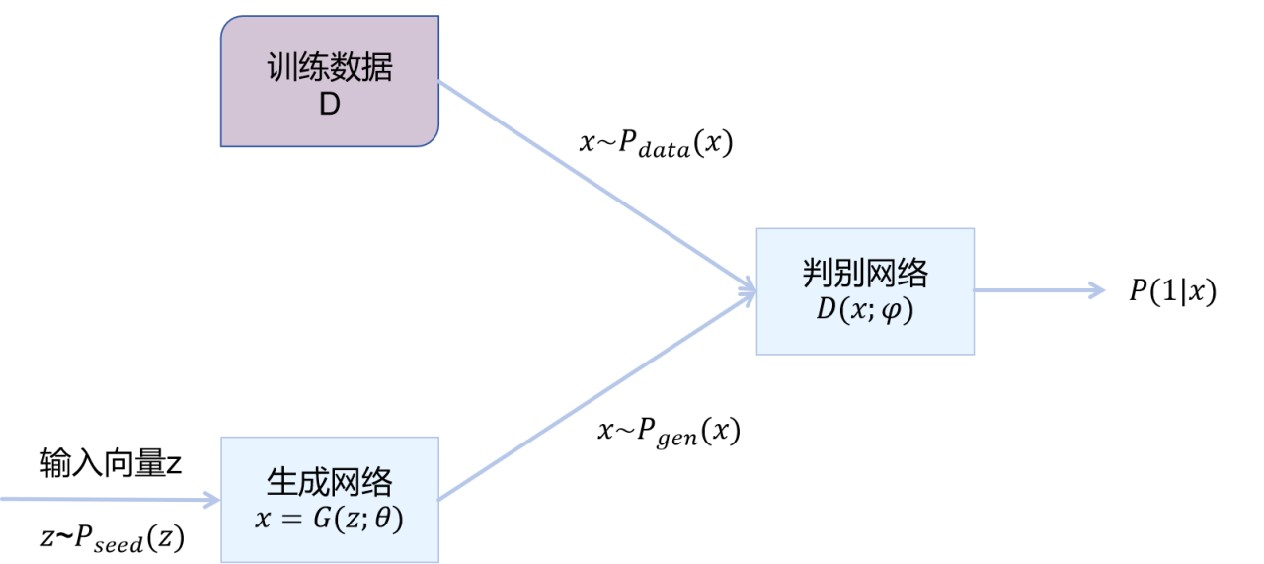
\includegraphics[width=10cm]{image/chap02/GAN.jpg}
    \caption{GAN的基础框架}
    \label{fig:GAN}
\end{figure}

判别网络和生成网络形成博弈关系,训练过程依赖与判别器的结果反馈,基于极大似然估计的思想,可以得到GAN的学习目标函数[附录补充]:
\begin{equation}
    \label{eq:example-formulas}
    V(G,D)=\underset{\theta}{\min}\underset{\phi}{\max}\Big[E_{x\sim P_{data}(x)}\log D(x;\phi)+E_{z\sim P_{seed}(z)}\log(1-D(G(z;\theta);\phi)]\Big]
\end{equation}

在GAN框架下,随着训练进行,生成器$G$生成图像质量越高,判别器$D$越可能误判,导致训练损失增加;判别器$D$判别能力越强,生成器$G$生成的图像更可能被打上“假”标签,训练损失增加。
最终两者在不断优化对抗下达到最优的对抗结果。在算法流程中,这种博弈关系体现为生成器与判别器交替进行神经网络的参数更新,参见\autoref{algo:GAN}。

\begin{algorithm}[h]
    \KwIn{训练集$\mathcal{D}$,对抗训练迭代次数$T$,每次判别网络的训练迭代次数$K$,小批量样本数量$M$}
    \For{$t\leftarrow 1$ \KwTo $T$}
    {
        //训练判别网络$D(x;\phi)$\\
        \For{$k\leftarrow 1$ \KwTo $K$}{
            //采集小批量训练样本\\
            从训练集$\mathcal{D}$中采集$M$个样本$\{x^{(m)}\},1\leq m\leq M$\\
            从分布$\mathcal{N}(\mathbf{0,I})$中采集$M$个样本$\{\mathbf{z}^{(m)},1\leq m\leq M\}$\\
            利用梯度下降法更新判别器网络参数
            \[
            \frac{\partial}{\partial \phi}\left[\frac{1}{M}\sum_{m=1}^M\left(log\ D(x^{(m)};\phi)+\log(1-D(G(z^{(m)};\theta);\phi))\right)\right]
            \]
        }
        //训练生成网络$G(z;\theta)$
        从分布$\mathcal{N}(\mathbf{0,I})$中采集$M$个样本$\{z^{(m)}\},1\leq m\leq M$\\
        利用梯度下降法更新生成器网络参数
        \[
        \frac{\partial}{\partial\theta}\left[\frac{1}{M}\sum_{m=1}^M D(G(z^{(m)};\theta),\phi)\right]
        \]
    }
    \KwOut{生成网络$G(z,\theta)$}
    \caption{生成对抗网络训练过程}
    \label{algo:GAN}
\end{algorithm}

\subsection{深度卷积生成对抗网络}
GAN的思想简单而深刻,在实际工程已有成熟的应用。本文实验主要基于一种广泛应用的GAN网络架构——深度生成对抗网络(Deep Convolutional GAN)。
DCGAN的研究成果\cite{radford2015unsupervised}发表于2015年。DCGAN基于GAN的思想,结合卷积神经网路,提出了全新的网络框架。DCGAN在训练中状态稳定,可以高质量地生成图片。并且展现了存在语义标签时,对图像生成结果的可控干扰。

DCGAN架构的设计规则主要聚焦于以下三点:

1)卷积层替代池化层:卷积神经网络(convolutional neural network)被证明可以有效捕捉图片特征,有助于网络下采样。

2)去除全连接层:减少网络参数量,尽可能避免过度对训练集的拟合,同时有助于加快网络训练速度

3)使用批归一化:批归一化(Batch normalization)对每一层的输入进行归一化处理,有效稳定数据分布。是一种加速训练并提高模型稳定性的技术。

\autoref{fig:DCGAN}展示了DCGAN中生成网络与判别网络架构。其中生成网络输入为长度100的潜在随机变量,而判别网络输出单一的判别结果。
\begin{figure}[!htbp]
    \centering
    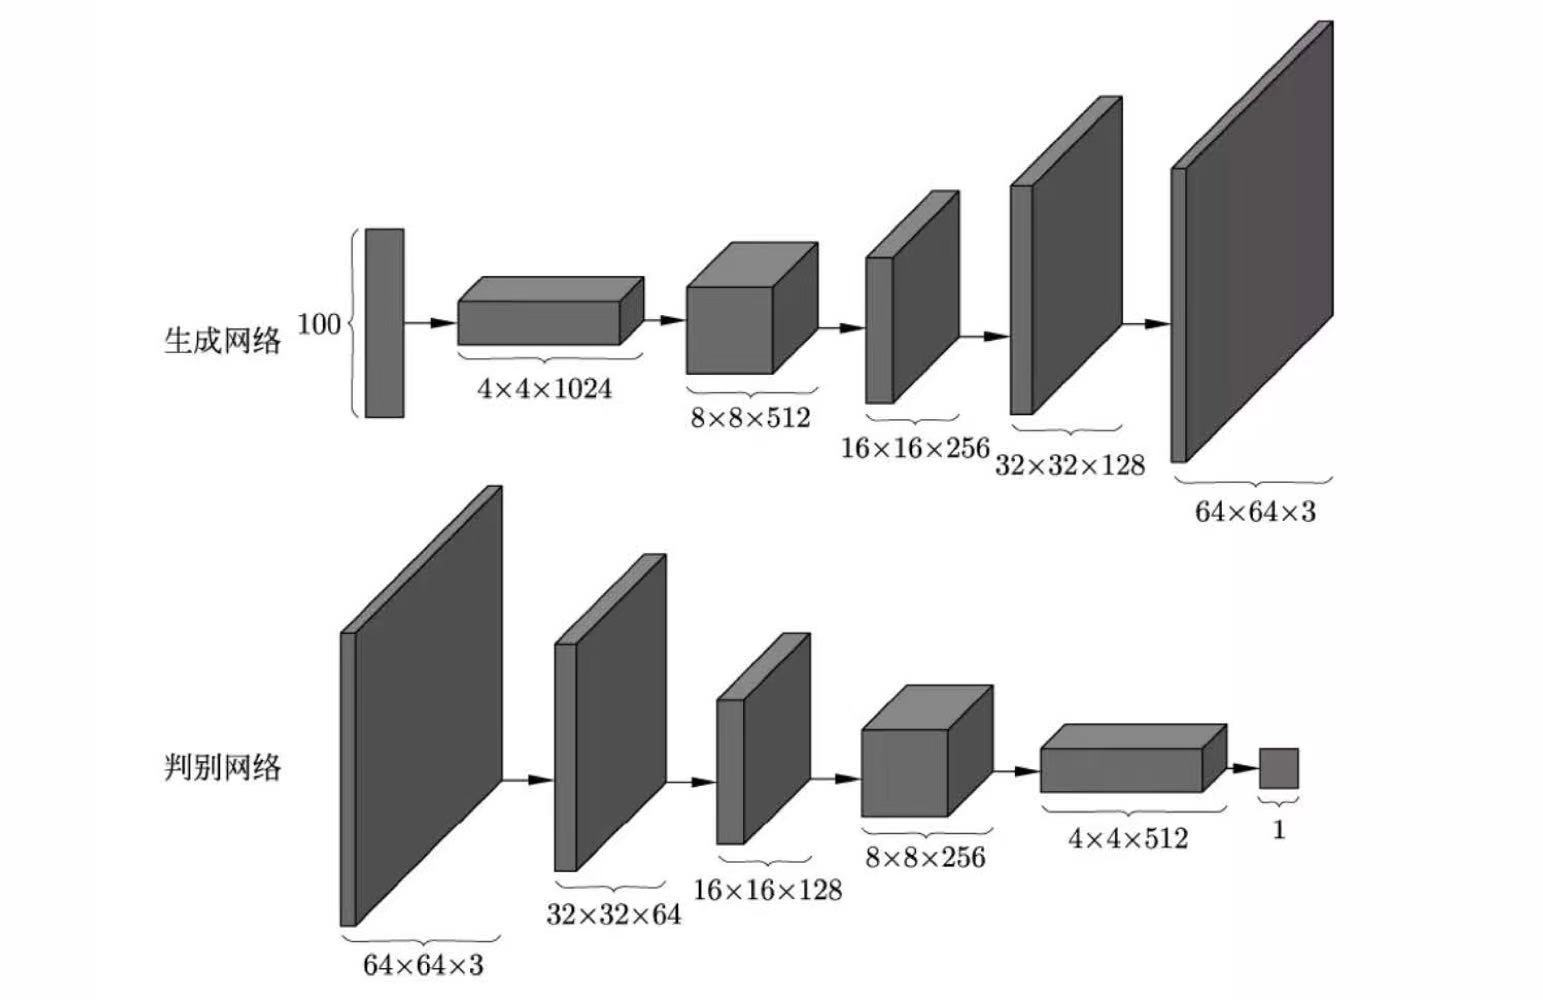
\includegraphics[width=10cm]{image/chap02/DCGAN.png}
    \caption{DCGAN网络结构}
    \label{fig:DCGAN}
\end{figure}

在实验中,生成对抗模型依然存在许多问题\cite{zhangtowards}。包括模式崩溃(生成器生成固定模式通过判别,生成样本失去多样性)、训练难度大(同时训练两个网络,存在多个超参数),解释性差(由于复杂博弈过程,图像生成过程缺乏解释性)。

\section{扩散模型}
扩散模型受热力学扩散过程的启发\cite{sohl2015deep},其目标是通过对数据点在潜空间中的扩散方式进行建模,来学习数据集的潜在结构。
扩散过程从数学角度来说就是:数据点的分布可以通过不断地添加噪声变成另一个分布。这种思路在图像生成任务中体现为:训练集的图像可以通过不断添加噪声,变成符合标准正态分布的图像(噪声)。
扩散模型通过神经网络学习添加噪声的过程,并可以实现加噪声的逆过程。在计算机视觉领域,这意味着可以通过学习逆扩散过程来训练神经网络,使其能对叠加了高斯噪声的图像进行去噪成像(从符合标准正态分布的噪声图像中去除噪声,得到图像)

扩散模型可以应用于各种任务,如图像去噪、图像修复、超分辨率成像、图像生成等等。Jonathan Ho等人在2020年论文《Denoising Diffusion Probabilistic Models》\cite{ho2020denoising}中利用扩散模型DDPM实现了高质量的图像生成,建立了前向加噪-反向降噪-训练的代码框架。
\subsection{前向过程}
在前向过程中,设定最大加噪次数的超参数$T$,对训练集的图像$x_0$添加$T$次噪声以使时刻$T$的图像$x_T$符合标准正态分布。
准确来说,\textbf{加噪声}并不是给$t-1$时刻的图像$\mathbf{x}_{t-1}$加上噪声值,而是从一个均值与图像$\mathbf{x}_{t-1}$相关的正态分布中采样新图像。
如\autoref{eq:sample}所示,$\mathbf{x}_{t-1}$是上一时刻的图像,$\mathbf{x}_t$是这一时刻生成的图像,该图像是从一个均值与$\mathbf{x}_{t-1}$有关的正态分布里采样出来的。
\begin{equation}
    \mathbf{x}_t\sim\mathcal{N}\Big(\mu_t(\mathbf{x}_{t-1}),\sigma_t^2\mathbf{I}\Big)
    \label{eq:sample}
\end{equation}
其中$x_t$只与上一时刻$x_{t-1}$有关,而与$x_{t-2},x_{t-3}...$无关,这说明前向过程是一个马尔科夫过程
\footnote{在概率论及统计学中,马尔可夫过程(Markov process)是一个具备了马可夫性质的随机过程,因为俄国数学家安德雷·马可夫得名。马尔可夫过程是不具备记忆特质的。换言之,马尔可夫过程的条件概率仅仅与系统的当前状态相关,而与它的过去历史或未来状态,都是独立、不相关的}。
这使得前向过程有良好的数学性质。
\begin{align*}
    \begin{split}
        q(x_1,...,x_T|x_0)=\prod_{t=1}^{T}q(x_t|x_{t-1})\\ 
        q(x_t|x_{t-1})=\mathcal{N}(x_t;\sqrt{1-\beta_t}x_{t-1},\beta_t\mathbf{I})
    \end{split}
\end{align*}

设置合适的加噪扩散次数$T$和具有特定性质的$\beta_t$,我们可以利用一步扩散公式得到从初始图像$x_0$得到任意时刻图像$x_t$的公式。详细推导可参考附录A
\begin{equation}
    x_t=\sqrt{\Pi_{i=1}^{t}(1-\beta_i)}x_0+\sqrt{1-\Pi_{i=1}^{t}(1-\beta_i)}
\end{equation}
为简化结果,令$\alpha_t=1-\beta_t,\overline{\alpha_t}=\prod_{i=1}^{t}\alpha_i$,可以得到$x_t$关于$x_0$的条件分布。
其中$1-\overline{\alpha_t}$反映了$t$时刻的此条件分布的方差。
\begin{equation}
    q(x_t|x_0)=\mathcal{N}(x_t;\sqrt{\bar{\alpha_t}},(1-\bar{\alpha_t})\mathbf{I})
\end{equation}

\subsection{反向过程}

正向过程设置了$T$步加噪声过程。在反向过程中,如果能够实现取消每一步加噪声操作,让一个纯噪声图像变成类似数据集的图像,就达到了图像生成的目标。
如何得到每一步的噪声,并且去除噪声,使得任意一个从标准正态分布里采样出来的噪声图像分布都能还原为训练集的图像分布。
扩散模型DDPM使用深度神经网络来预测每一步的噪声,并进行去噪声操作。数学原理表明[附录补充],当$\beta_t$足够小时,每一步加噪声的逆操作也满足正态分布。
\begin{equation}
    \mathbf{x}_{t-1}\sim\mathcal{N}(\tilde{\mu_t},\tilde{\beta_t}\mathbf{I})
\end{equation}
其中,当前时刻加噪声逆操作的均值$\tilde{\mu_t}$和方差$\tilde{\beta_t}$由当前时刻$t$,当前的图像$x_t$决定。
因此,为了描述所有去噪声操作,神经网络需要输入$t$,$x_t$,拟合前一步图像$\mathbf{x}_{t-1}$服从分布的均值$\tilde{\mu_t}$和方差$\tilde{\beta_t}$。

在理想情况下,去操作就等于加噪声操作的逆操作。DDPM模型使用神经网络拟合噪声,这反映\textbf{去噪声}和\textbf{加噪声逆操作}的关系
就是神经网络的\textbf{预测值}和\textbf{真值}的关系。从概率分布的角度来说就是,如何尽可能使条件分布$q(\mathbf{x}_t|\mathbf{x}_{t-1})$接近$p_{\theta}(\mathbf{x}_{t-1}|\mathbf{x}_t)$,参见\autoref{fig:DDPM}。
\begin{figure}[!htbp]
    \centering
    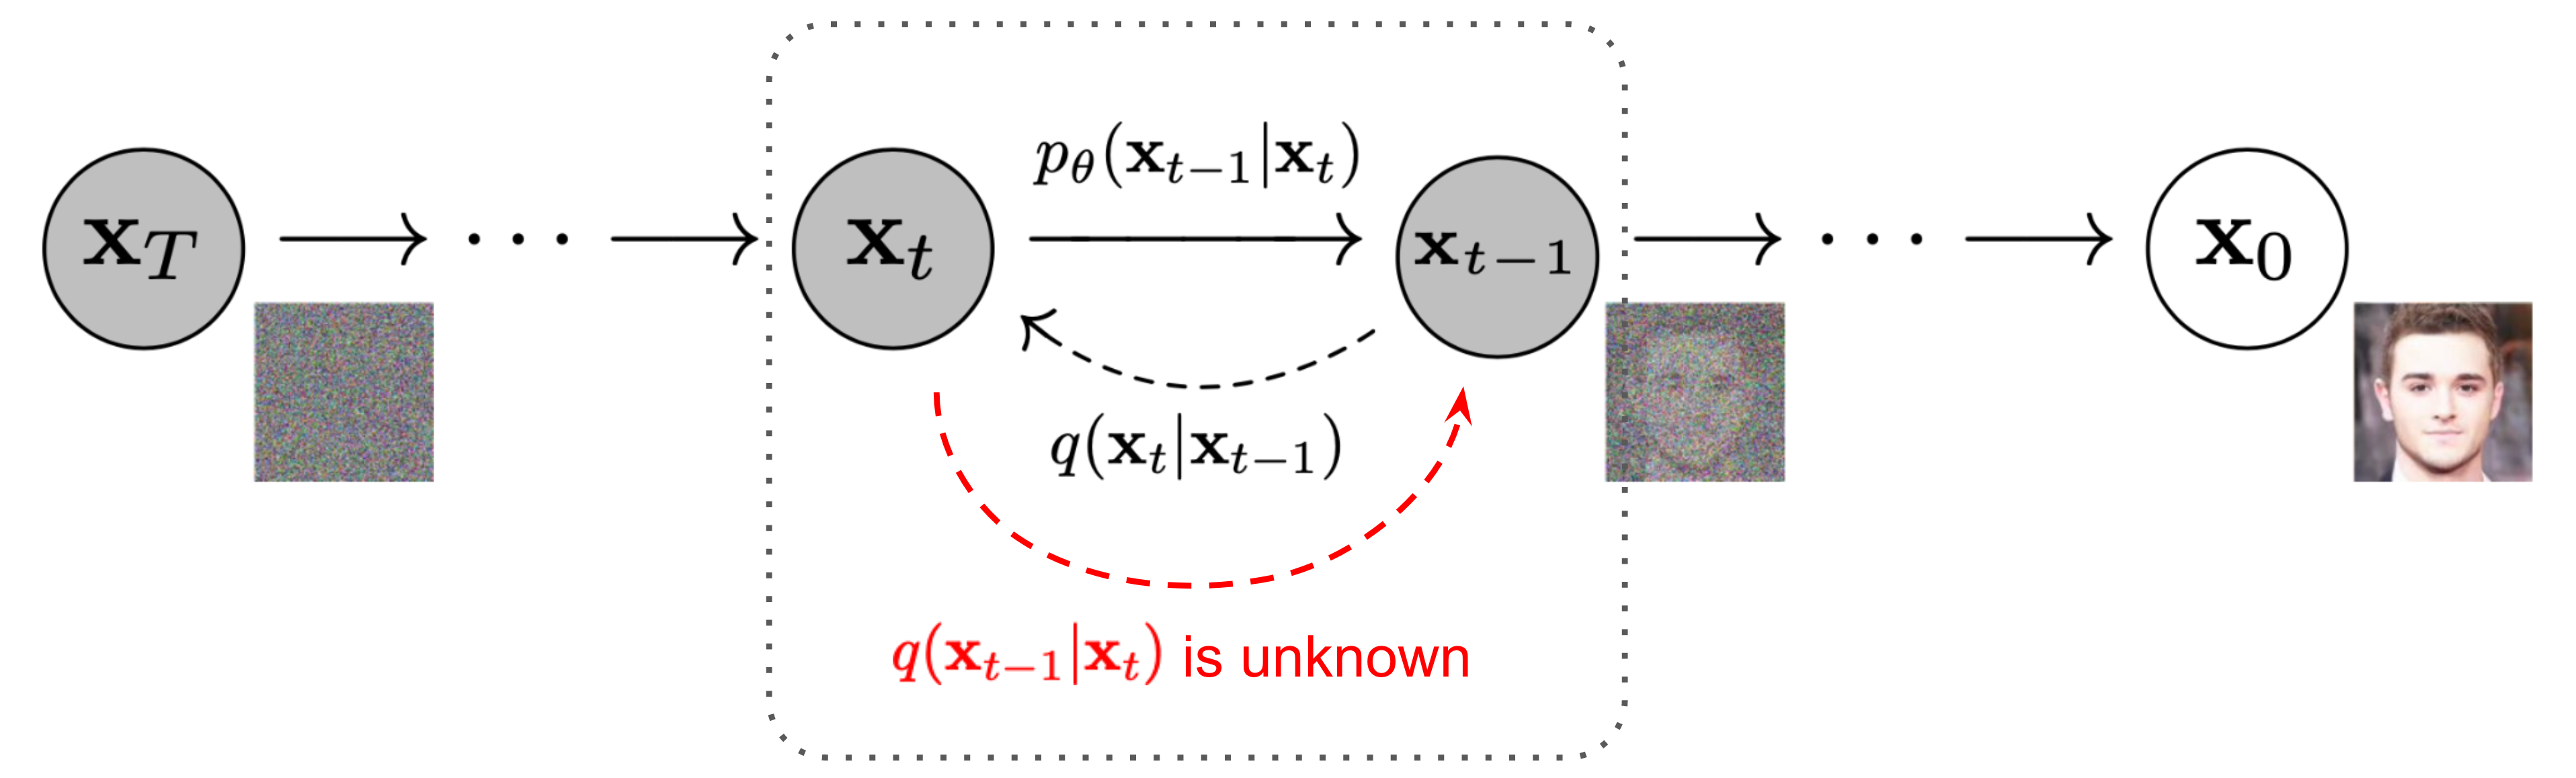
\includegraphics[width=10cm]{image/chap02/DDPM.png}
    \caption{DDPM示意图}
    \label{fig:DDPM}
\end{figure}
然而,直接计算所有数据的加噪声逆操作的分布是困难的。但若给定了训练集输入$x_0$,利用贝叶斯公式可以计算得到
$$
q(x_{t-1}|x_t,x_0)=q(x_t|x_{t-1},x_0)\dfrac{q(x_{t-1}|x_0)}{q(x_t|x_0)} 
$$
在上面的等式中,左边的$q(x_{t-1}|x_t,x_0)=\mathcal{N}(x_{t-1};\tilde{\mu_t},\tilde{\beta_t}\mathbf{I})$表示加噪声操作的逆操作,它的均值和方差都是待求的。
右边的$q(x_t|x_{t-1},x_0)=\mathcal{N}(x_t;\sqrt{1-\beta_t}x_{t-1},\beta_t\mathbf{I})$是加噪声的分布。
由于$\mathbf{x_0}$已知,$q(x_{t-1}|x_0)$和$q(x_t|x_0)$两项可以根据公式$x_t=\sqrt{\bar{\alpha_t}}x_0+\sqrt{1-\bar{\alpha_t}}\epsilon_t$得到:
\begin{equation}
    \begin{split}
        q(x_t|x_0)=\mathcal{N}(x_t;\sqrt{\bar{\alpha_t}}x_0,(1-\bar{\alpha_t})\mathbf{I}) \\
        q(x_{t-1}|x_0)=\mathcal{N}(x_{t-1};\sqrt{\bar{\alpha}_{t-1}}x_0,(1-\bar{\alpha}_{t-1})\mathbf{I})
    \end{split}
\end{equation}
这样等式右边的式子全部已知。将上式代入可以算出给定$x_0$时的去噪声分布。经计算[附录补充]化简,分布的均值$\tilde{\mu_t}$和方差$\tilde{\beta_t}$
\begin{equation}
    \label{eq:mean}
    \tilde{\mu_t}=\frac{1}{\sqrt{\alpha_t}}(x_t-\frac{1-\alpha_t}{\sqrt{1-\bar{\alpha_t}}}\epsilon_t)
\end{equation}
其中$\epsilon_t$是从标准正态分布采样处的样本。
\begin{equation}
    \tilde{\beta_t}=\frac{1-\bar{\alpha}_{t-1}}{1-\bar{\alpha_t}}\beta_t
\end{equation}
分布的方差与输入$x_0$无关,因此在训练神经网络进行去噪时,只需要拟合$T$步中各时刻均值即可,方差则由噪声方差$\beta_t$决定。
在利用去噪网络拟合均值时,参见\autoref{eq:mean},去噪过程中$\mathbf{x}_t$是已知的。唯一不确定是$\epsilon_t$。
所用设置的神经网络只需要预测噪声$\epsilon_{\theta}(\mathbf{x}_t,t)$(其中$\theta$为可学习参数)即可。

设置$\epsilon_{\theta}(\mathbf{x}_t,t)$和生成$\mathbf{x}_t$的噪声$\epsilon_t$的均方误差MSE最小即可。因此对于一轮训练,最终的损失函数可写成[附录补充]
\begin{equation}
    \mathbf{L}=\big|\big|\epsilon_t-\epsilon_{\theta}(x_t,t)\big|\big|^2
\end{equation}

\subsection{神经网络选择}
扩散模型DDPM的前向过程和反向过程,在算法流程中体现为训练神经网络\autoref{algo:train}和采样生成图像\autoref{algo:denoise}两部分。
\begin{algorithm}[h]
    \KwIn{训练集样本$x_0$}
    \While{损失函数未收敛到指定精度时}{
        \[
        t\sim\ Uniform(\{1,...,T\}),
        \epsilon\sim\mathcal{N}(\mathbf{0},\mathbf{I})
        \]
        利用梯度下降法更新去噪神经网络
        \[
        \nabla_{\theta}\big|\big|\epsilon-\epsilon_{\theta}(\sqrt{\bar{\alpha}_t}x_0+\sqrt{1-\bar{\alpha}_t\epsilon,t})\big|\big|^2
        \]
    }
    \caption{算法1:训练拟合噪声}
    \label{algo:train}
\end{algorithm}
在\autoref{algo:train}中,$\epsilon_{\theta}(x_t,t)$是一个神经网络的映射,输入图像$\mathbf{x}_t$和时间$t$输出噪声预测。
在DDPM中并没有规定神经网络要求,通常会根据图像生成任务的难易程度,定义简单或复杂的网络结构。
原始论文中\cite{ho2020denoising},所用神经网络是经典的U-Net网络
\footnote{U-Net最早是用于生物医学图像分割开发的卷积神经网络\cite{ronneberger2015u}。其基于完全卷积网络,并在结构上加以修改与扩展,使得它可以用更少的训练图像产生更精确的分割。
U-Net架构已经在扩散模型中采用,用于迭代式图像去噪音。该网络网络由一个收缩路径(contracting path)和一个扩展路径(expansive path)组成,使其具有U形结构。}。
\begin{algorithm}[h]
    \KwIn{噪声样本$x_T\sim\mathcal{N}(\mathbf{0},\mathbf{I})$}
    \For{$t=T,...,1$}{
        \[
        z\sim\mathcal{N}(\mathbf{0},\mathbf{I})if\ t>1,else\ z=0 
        \]
        \[
        x_{t-1}=\frac{1}{\sqrt{\alpha_t}}\left(x_t-\frac{1-\alpha_t}{\sqrt{1-\bar{\alpha_t}}}\epsilon_{\theta}(x_t,t)+\sigma_t\ Z\right)
        \]
    }
    \KwOut{拟合训练集的生成图像$\hat{x_0}$}
    \caption{算法2:去噪声生成图像过程}
    \label{algo:denoise}
\end{algorithm}

训练结束后,可以利用去噪声算法生成图像。由于$x_T$是从标准正态分布里随机采样的输入噪声,可以通过选取不同初始噪声,得到不同的图像生成结果,满足图像多样性的需求。
\newclearpage
\chapter{\LaTeX 模板配置与使用}


\label{cha:sysu-thesis-latex-install-guide}

本部分内容将让你能够通过本\LaTeX 模板生成一份可用的pdf,并为后面修改源码撰写毕设做准备。

首先,我们会展示最简单的方法:直接使用overleaf进行编写。然后,我们整理了不同环境下\LaTeX 环境的配置指南与不同写作工具的配置技巧,方便各位同学使用本\LaTeX 模板。最后,我们说明了如何开始编写自己的毕业论文(设计)。


\section{使用Overleaf编写毕设}

Overleaf\footnote{网址可见\url{https://www.overleaf.com/}}是一个在线的Latex文档协作平台。我们不需要配置任何环境,便能够在上面直接使用本模板进行写作。操作步骤如下:

第一步,下载本项目压缩包(从\url{https://github.com/SYSU-SCC/sysu-thesis/releases}处下载即可),注意需要下载zip格式的压缩包。
然后,我们在Overleaf上新建项目,并上传该压缩包,可参考\autoref{fig:overleaf-new-proj}。


\begin{figure}[h]
	\centering
	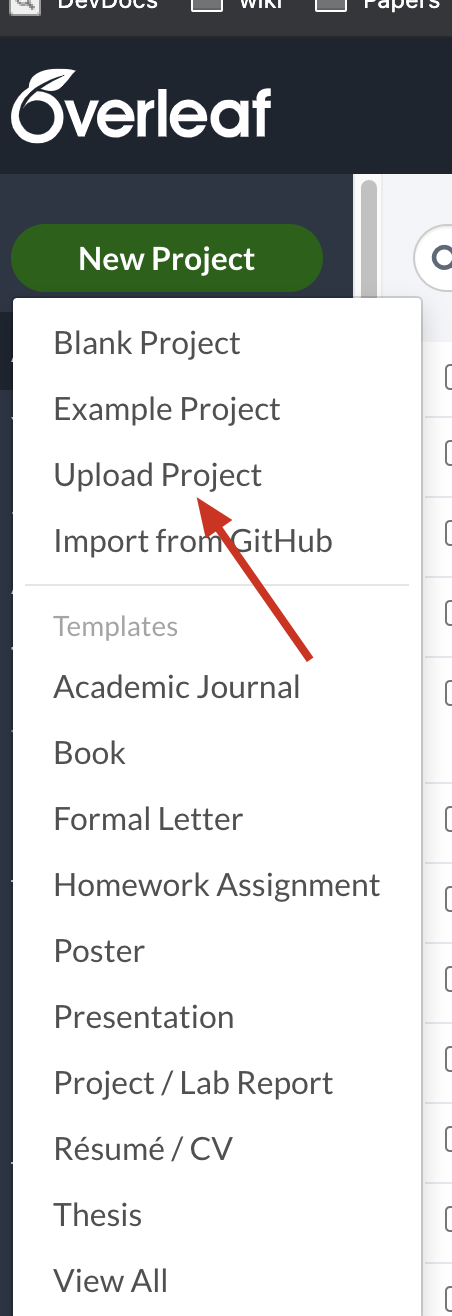
\includegraphics[width=0.2\textwidth]{image/chap03/overleaf-create-proj.jpg}
	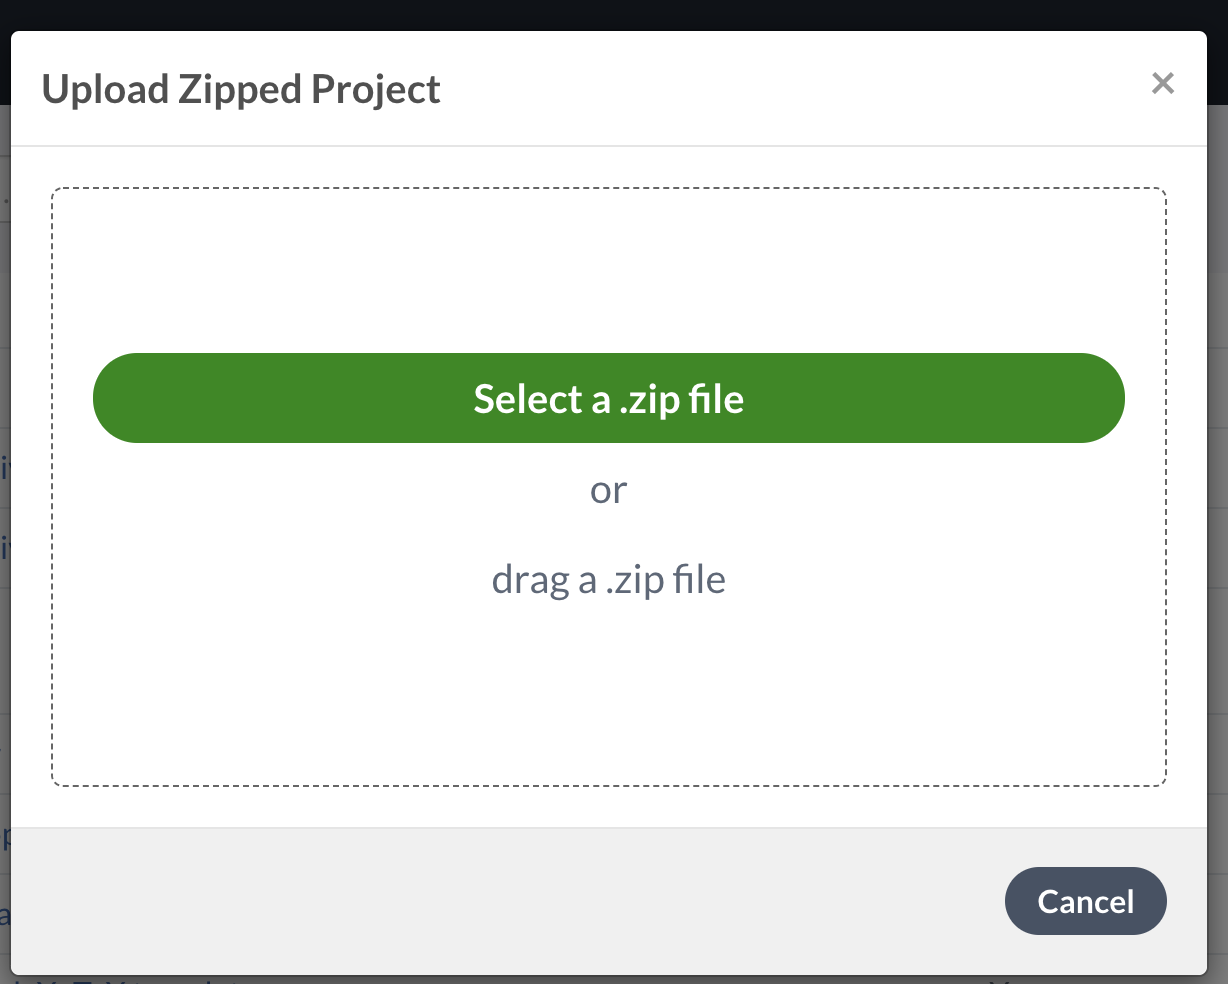
\includegraphics[width=0.7\textwidth]{image/chap03/overleaf-upload-proj.jpg}
	\caption{在Overleaf上创建并上传压缩包。}
	\label{fig:overleaf-new-proj}
\end{figure}

第二步,在Overleaf的菜单中调整编译工具为\texttt{xelatex},可参考\autoref{fig:overleaf-config}。

\begin{figure}[h]
	\centering
	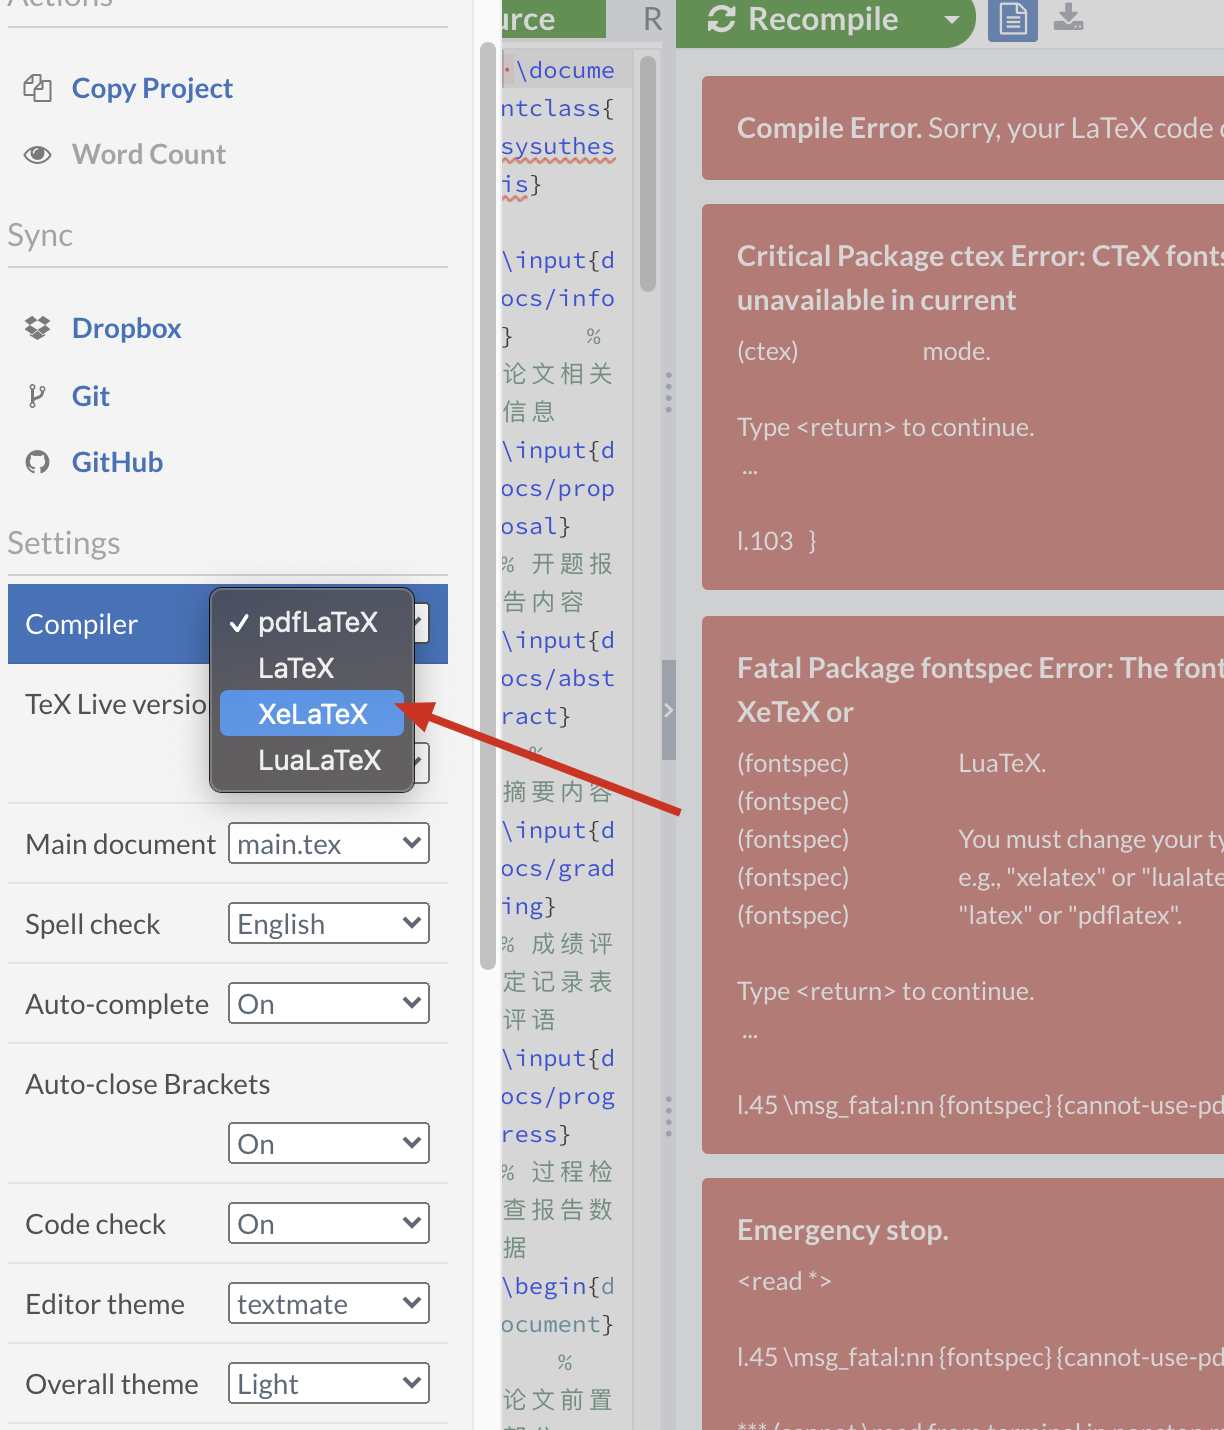
\includegraphics[width=0.6\textwidth]{image/chap03/overleaf-config.jpg}
	\caption{在Overleaf上调整编译工具}
	\label{fig:overleaf-config}
\end{figure}


第三步,点击编译,得到本pdf,可以开始修改pdf了!最终可见\autoref{fig:overleaf-example}。


\begin{figure}[h]
	\centering
	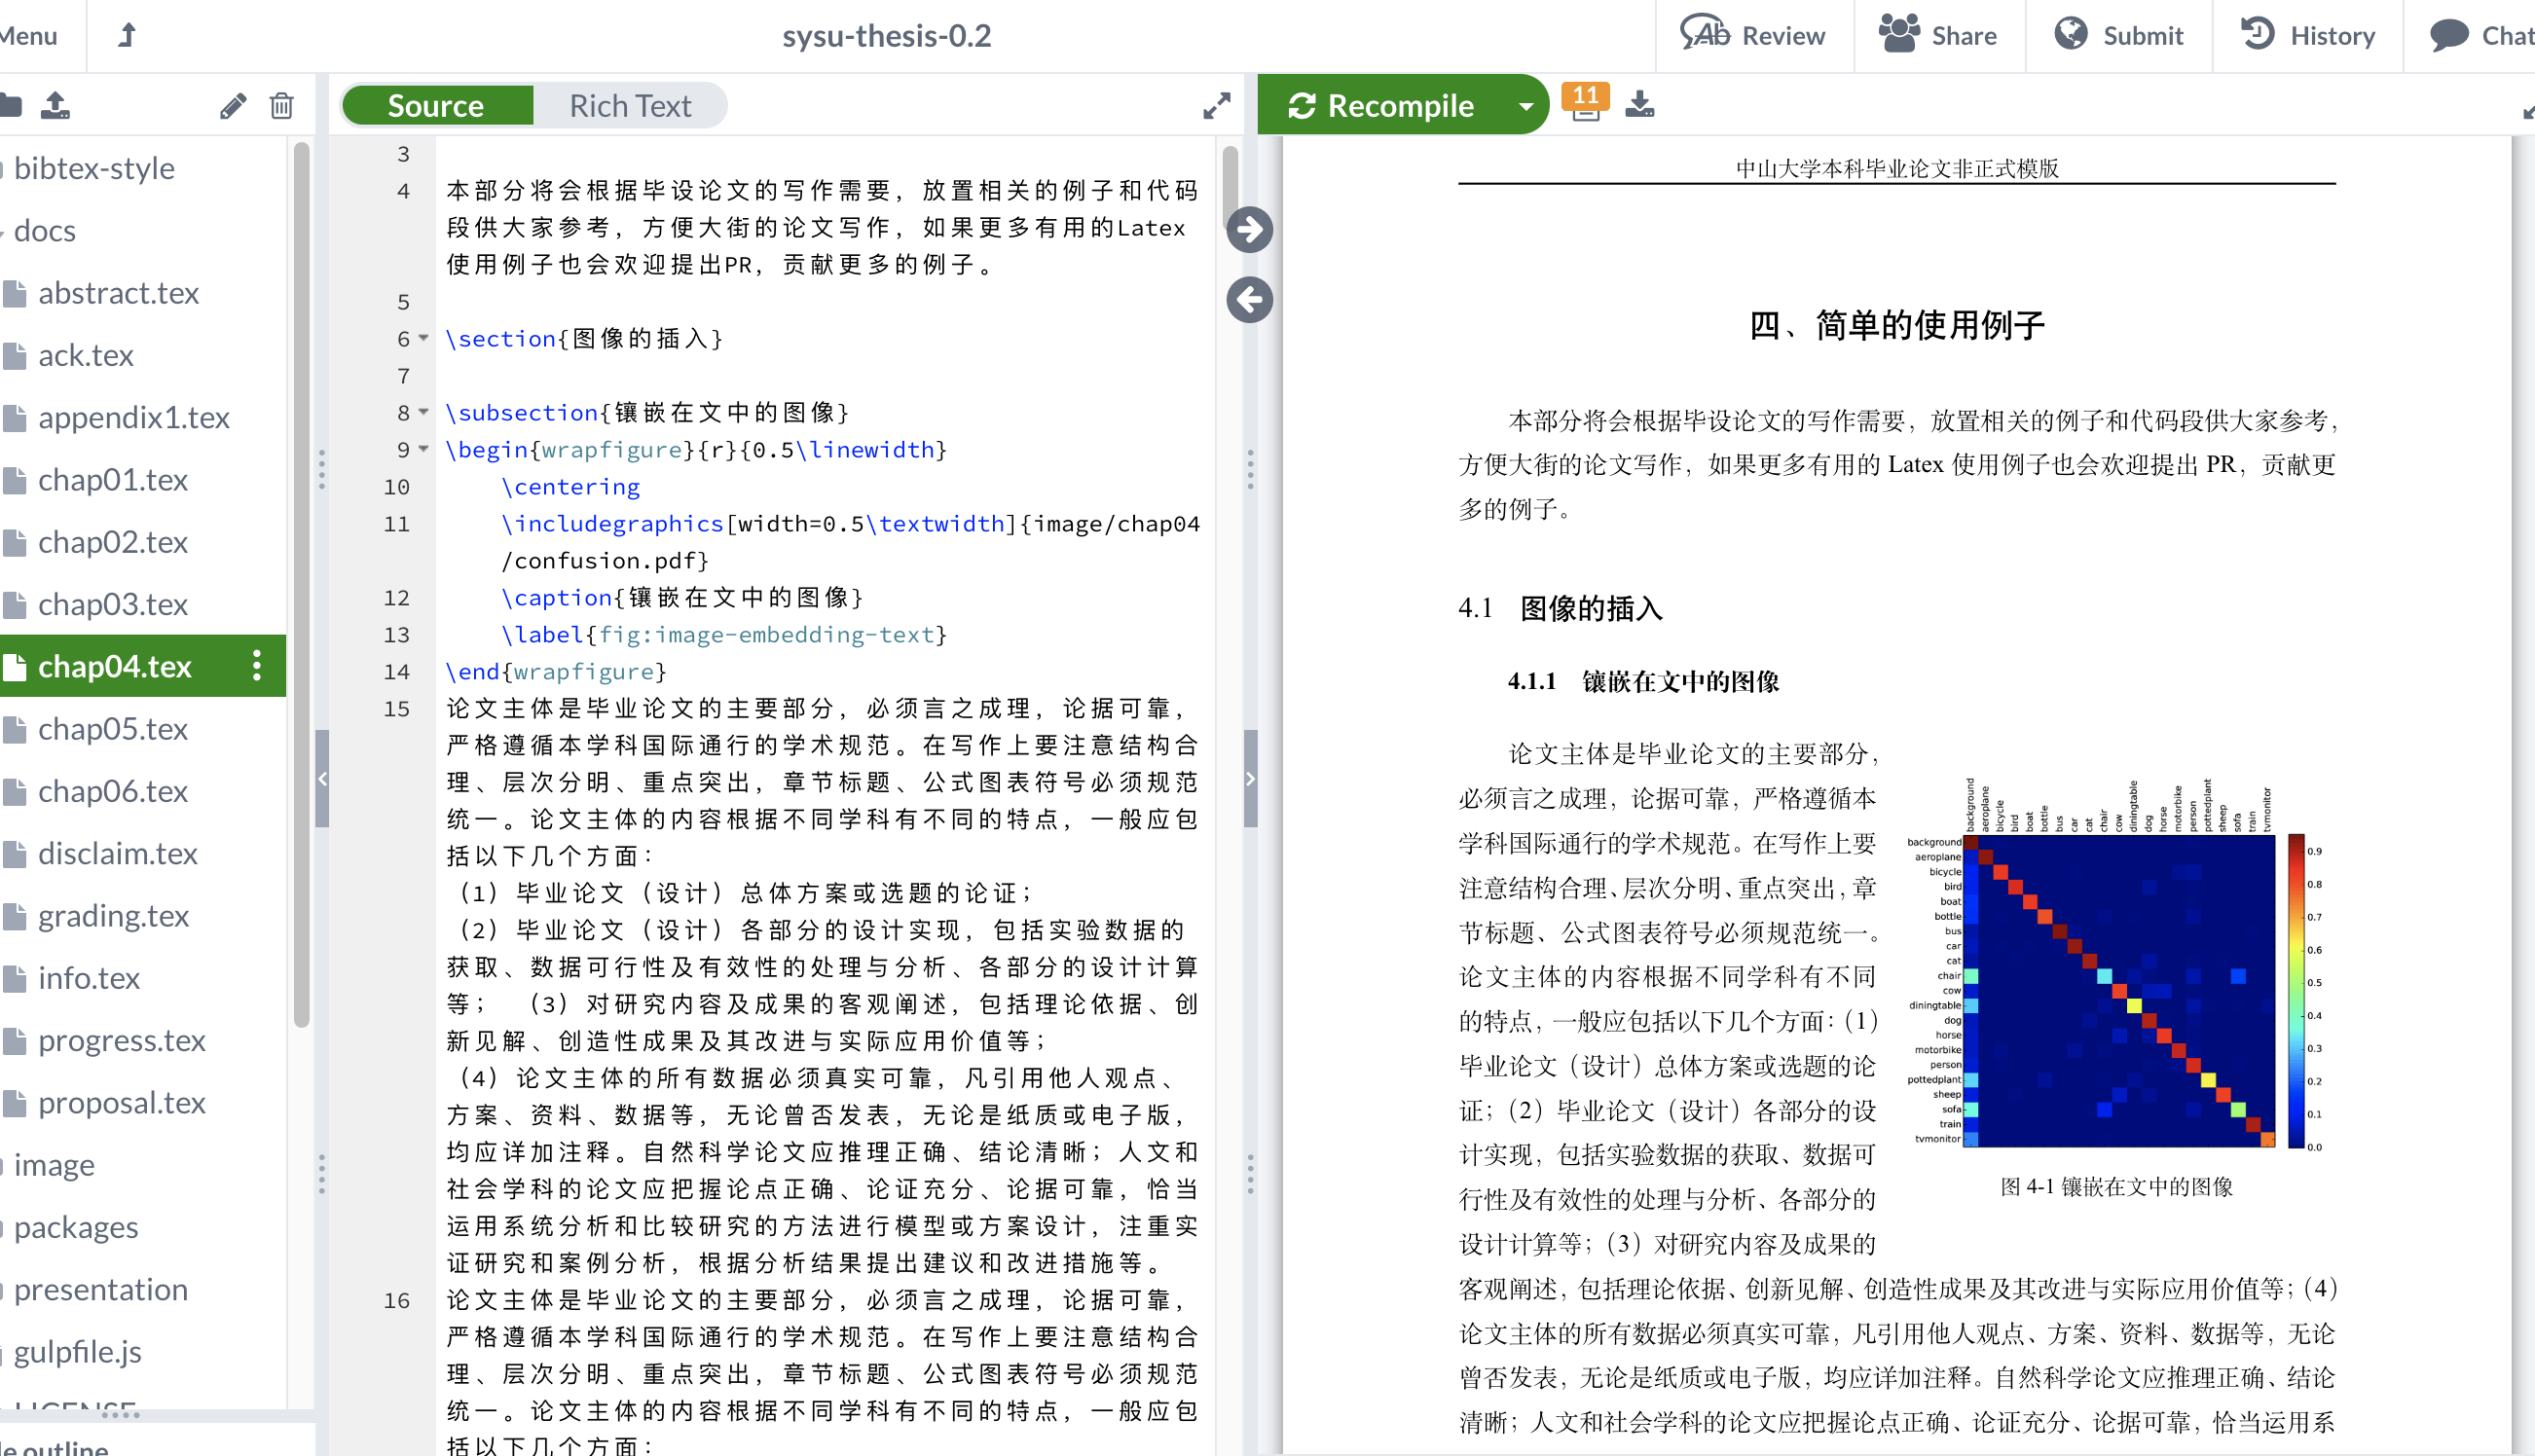
\includegraphics[width=0.9\textwidth]{image/chap03/overleaf-example.jpg}
	\caption{Overleaf使用例子}
	\label{fig:overleaf-example}
\end{figure}



\section{编译环境配置}

编译环境配置相对来说比较简单,下载Tex Live2020并如同一般的程序一样安装即可。

\subsection{编译环境配置:Window篇}

在\url{https://mirrors.tuna.tsinghua.edu.cn/CTAN/systems/texlive/Images/}上下载Tex Live2020并参考教程\footnote{可以参考\url{https://zhuanlan.zhihu.com/p/58811994}}安装即可。

\subsection{编译环境配置:Linux篇}

在\url{https://mirrors.tuna.tsinghua.edu.cn/CTAN/systems/texlive/Images/}上下载Tex Live2020并参考教程\footnote{可以参考\url{https://zhuanlan.zhihu.com/p/55894177}}安装即可。


\subsection{编译环境配置:MacOS篇}

在MacOS上配置Latex的环境,这里我们使用的是MacTex。

\begin{enumerate}
	\item \url{https://www.tug.org/mactex/}下载MacTex安装。
	\item 安装步骤:不详细展开,按照图形界面点击即可, 傻瓜式安装。
\end{enumerate}

TIPS:MacTex文件比较大,有2G多,介意的话可以选择MacTex\_Basic包,只有100M以内,但是如果安装MacTex\_Basic,后期可能会遇到各种缺包的问题。


安装完成之后,可以简单测试一下安装是否成功。如可以查看Texshop应用是否安装好,或者在命令行测试一下\texttt{xelatex}命令是否可用。

\section{写作环境配置}

不同的写作工具对应不同的写作环境。这里我们给出几个工具的配置例子以供参考。

\subsection{模板编译流程}

由于\LaTeX 的限制,本模板需要经过四次编译才能生成完整的论文:

\begin{enumerate}
	\item 先使用xelatex编译一次
	\item 再使用bibtex编译一次
	\item 然后使用xelatex编译两次
\end{enumerate}

本编译流程已经写在Makefile中,修改模板源码后只需要执行\texttt{make pdf}即可按照该流程进行编译并生成最终的pdf。



\subsection{写作环境配置:Visual Studio Code}

Visual Studio Code是微软公司推出的轻量代码编辑器,我们可以做一些简单的配置,便可以用该编辑器修改我们的\LaTeX 模板,并实现一键编译。

\begin{enumerate}
	\item 安装 Visual Studio Code。
	\item 安装 LaTeX Workshop 插件。
\end{enumerate}

本项目的\texttt{.vscode/setting.json}下已经包含了与前面所述编译流程相同的配置。正常配置下,每次修改模板源码后按下保存(Ctrl+S),就能够自动进行编译产生pdf。效果图如\autoref{fig:vscode-example}所示。


\begin{figure}[h]
	\centering
	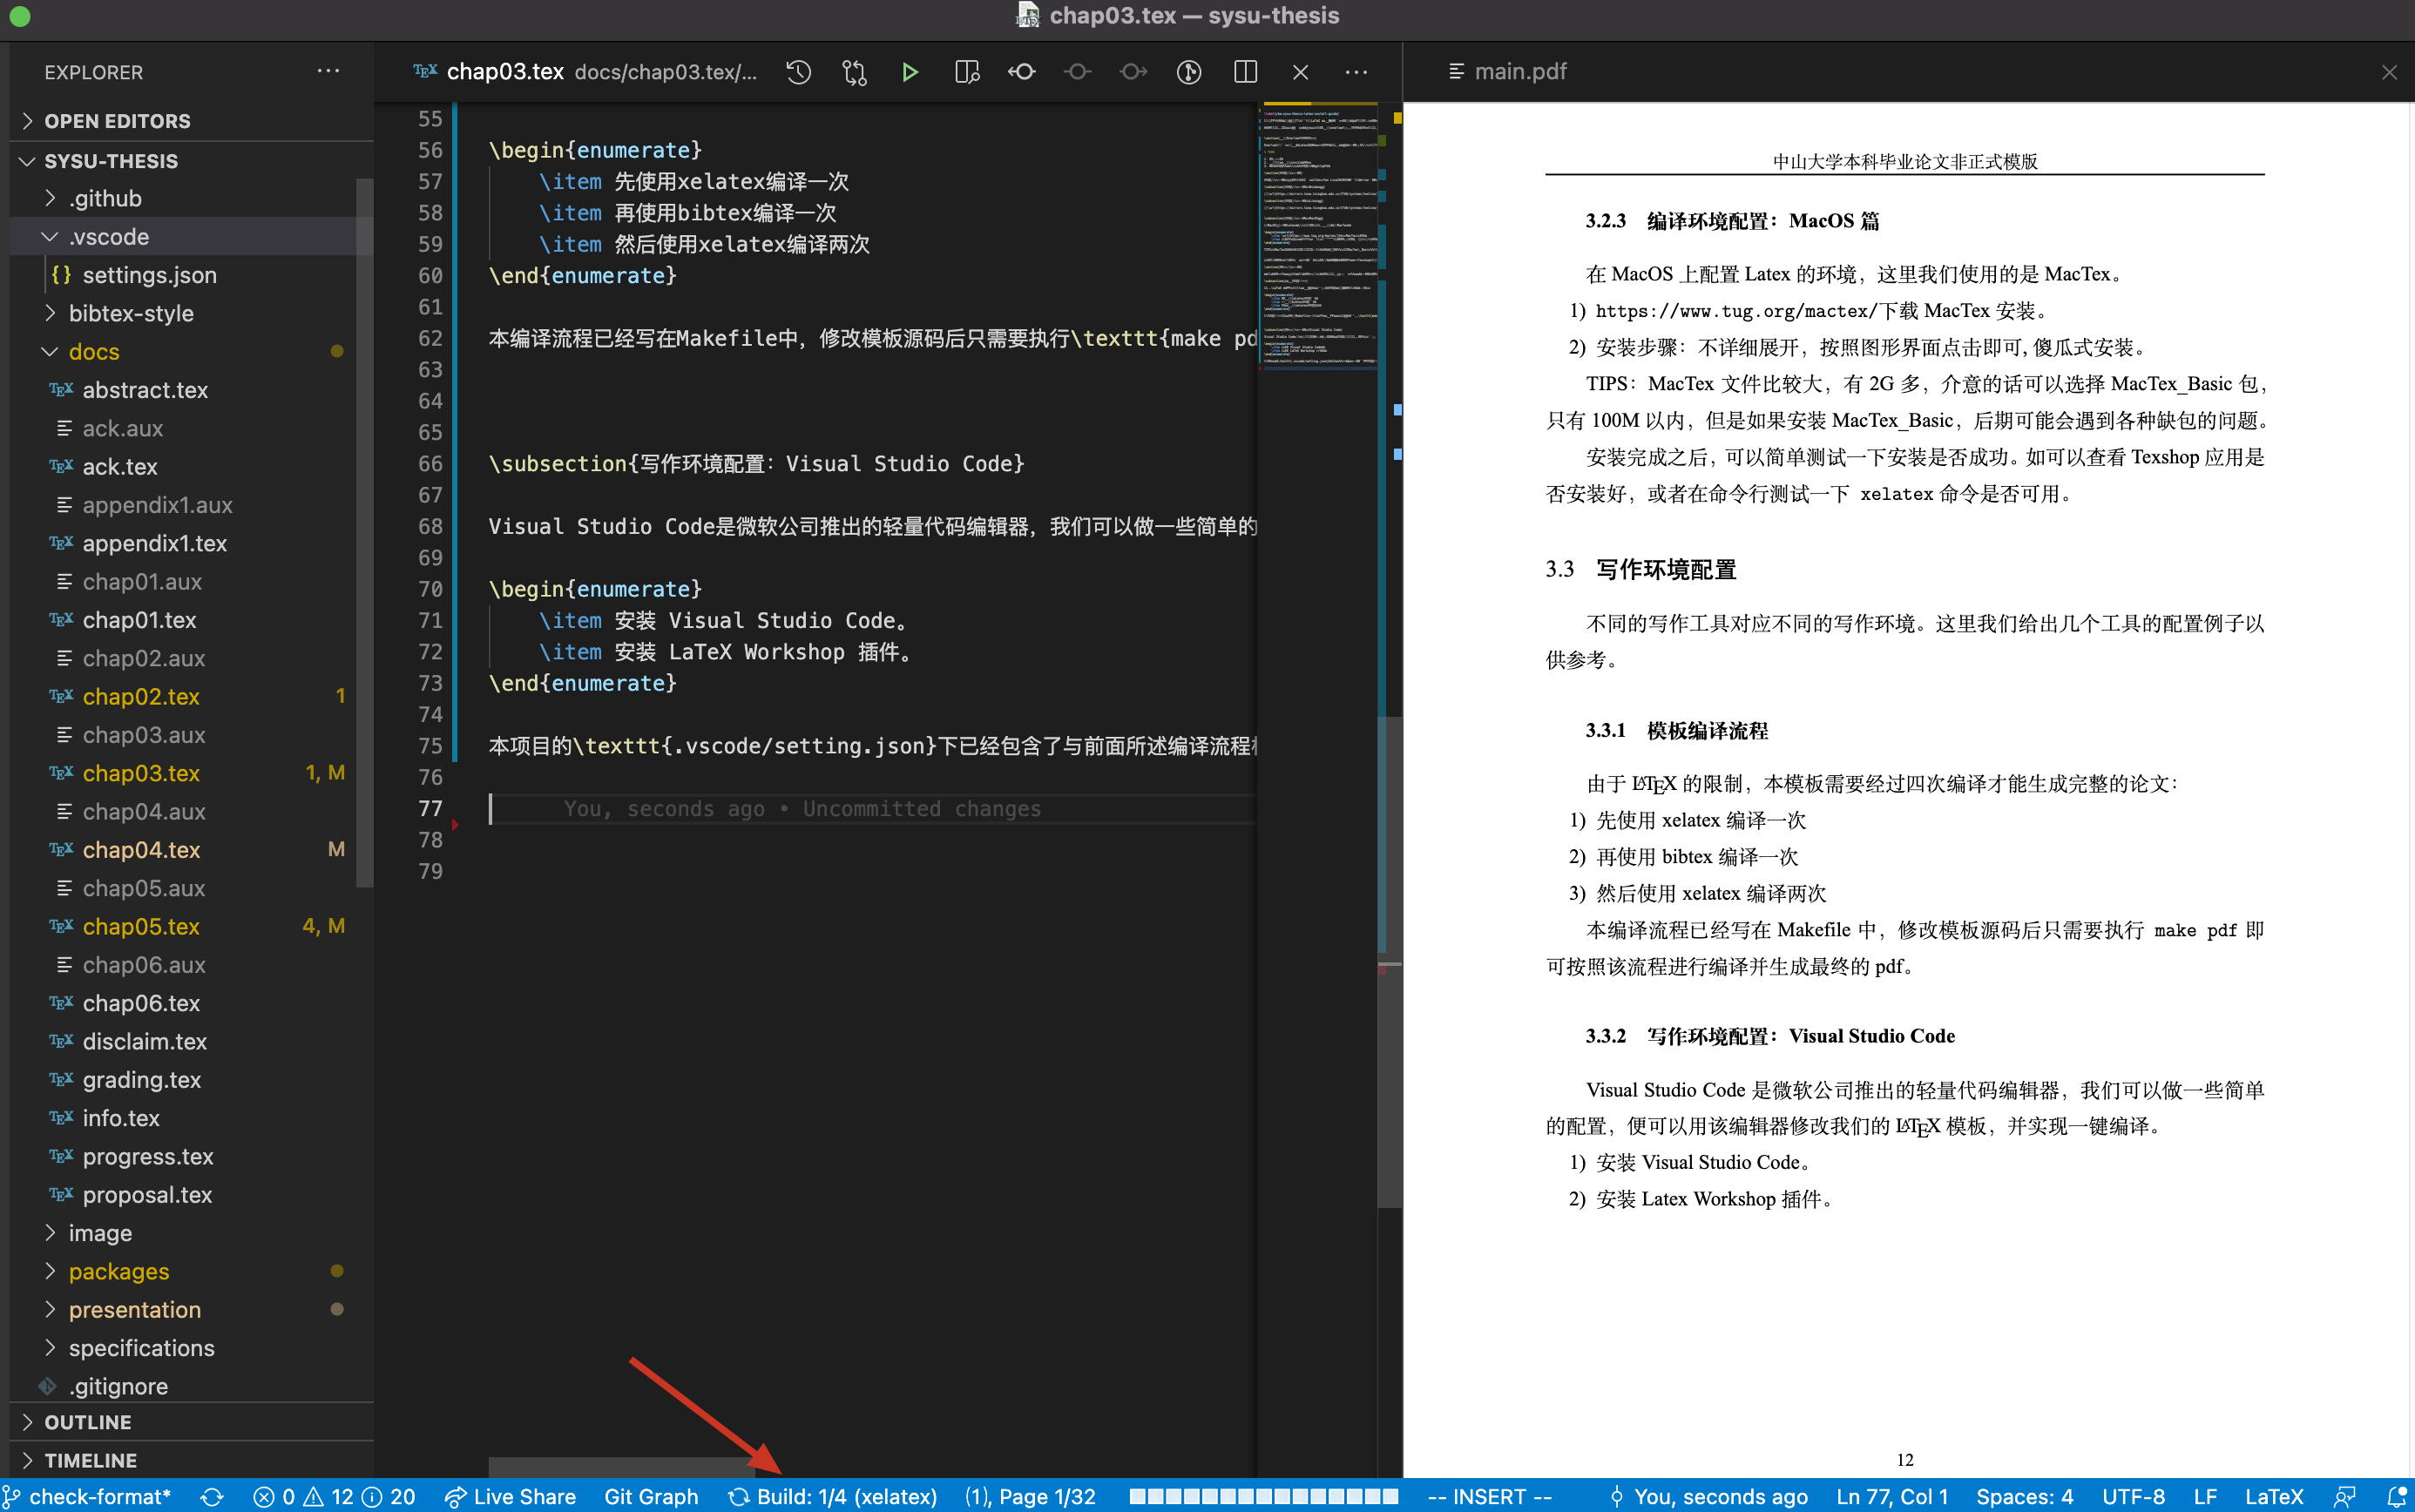
\includegraphics[width=\linewidth]{image/chap03/vscode-example.png}
	\caption{vscode配置好后的样例}
	\label{fig:vscode-example}
\end{figure}


\section{如何开始写毕业论文(设计)}

首先将所有个人信息,包括学号、姓名、专业、论文题目等,在\texttt{./docs/info.tex}中逐项进行更新。

然后我们再编辑\texttt{./docs/abstract.tex}补充论文摘要。

到了论文主体部分,我们可以自行编辑\texttt{./docs/chap01.tex},\texttt{./docs/chap02.tex}等文件进行编辑。如果章数不够,可以自行修改\texttt{main.tex}增加新的章节。

当论文主体编写完成后,我们再编辑\texttt{./docs/ack.tex}作为论文致谢。


% 首先将个人信息写到\texttt{./docs/info.tex}中。
\newclearpage
\chapter{简单的使用例子}
\label{cha:usage-example}

本部分将会根据毕设论文的写作需要,放置相关的例子和代码段供大家参考,方便大家的论文写作,如果更多有用的Latex使用例子也会欢迎提出PR,贡献更多的例子。

\section{图像的插入}

\subsection{镶嵌在文中的图像}
\begin{wrapfigure}{r}{0.5\linewidth}
    \centering
    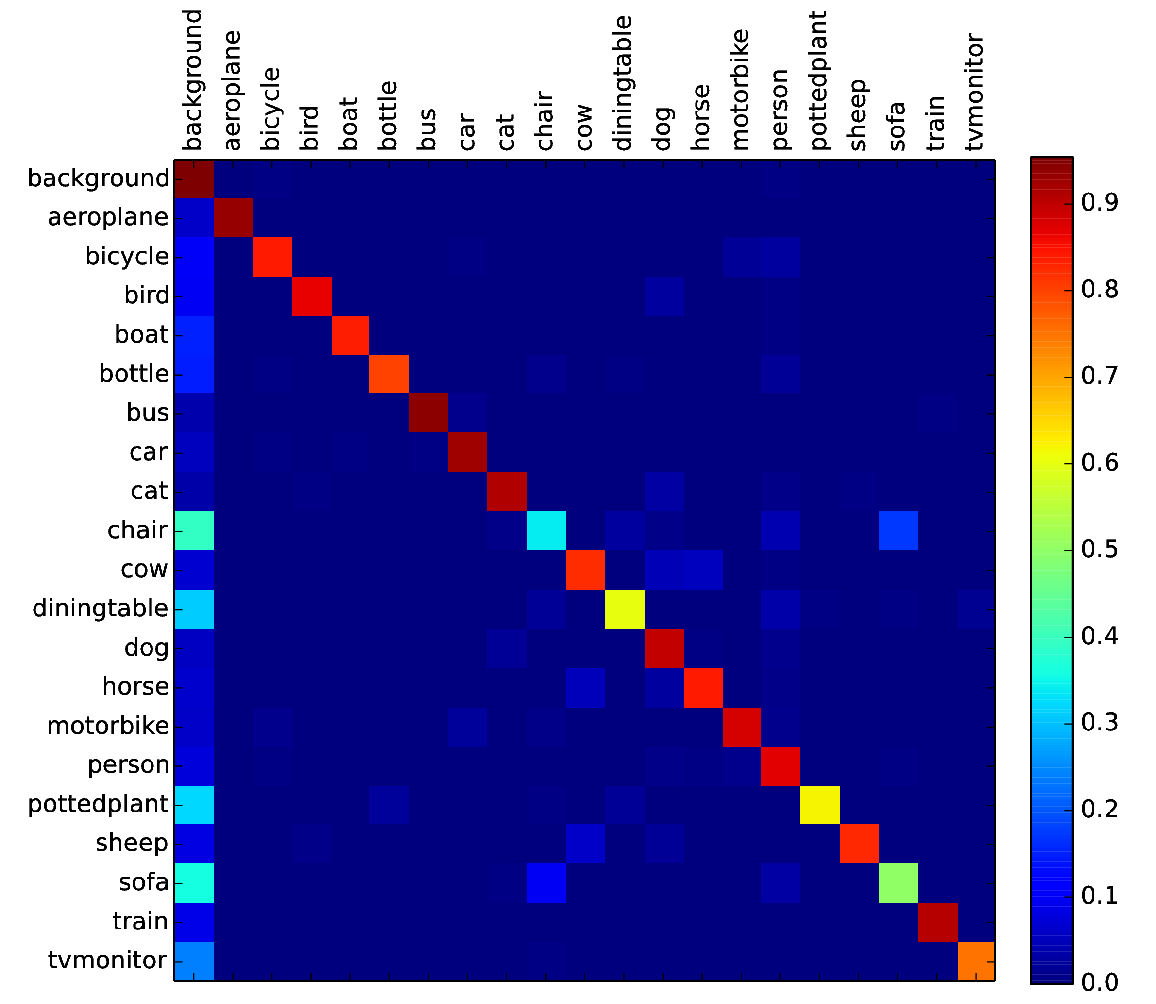
\includegraphics[width=0.5\textwidth]{image/chap04/confusion.pdf}
    \caption{镶嵌在文中的图像}
    \label{fig:image-embedding-text}
\end{wrapfigure}

\subsection{单张图像的插入}

\begin{figure}[h]
    \centering
    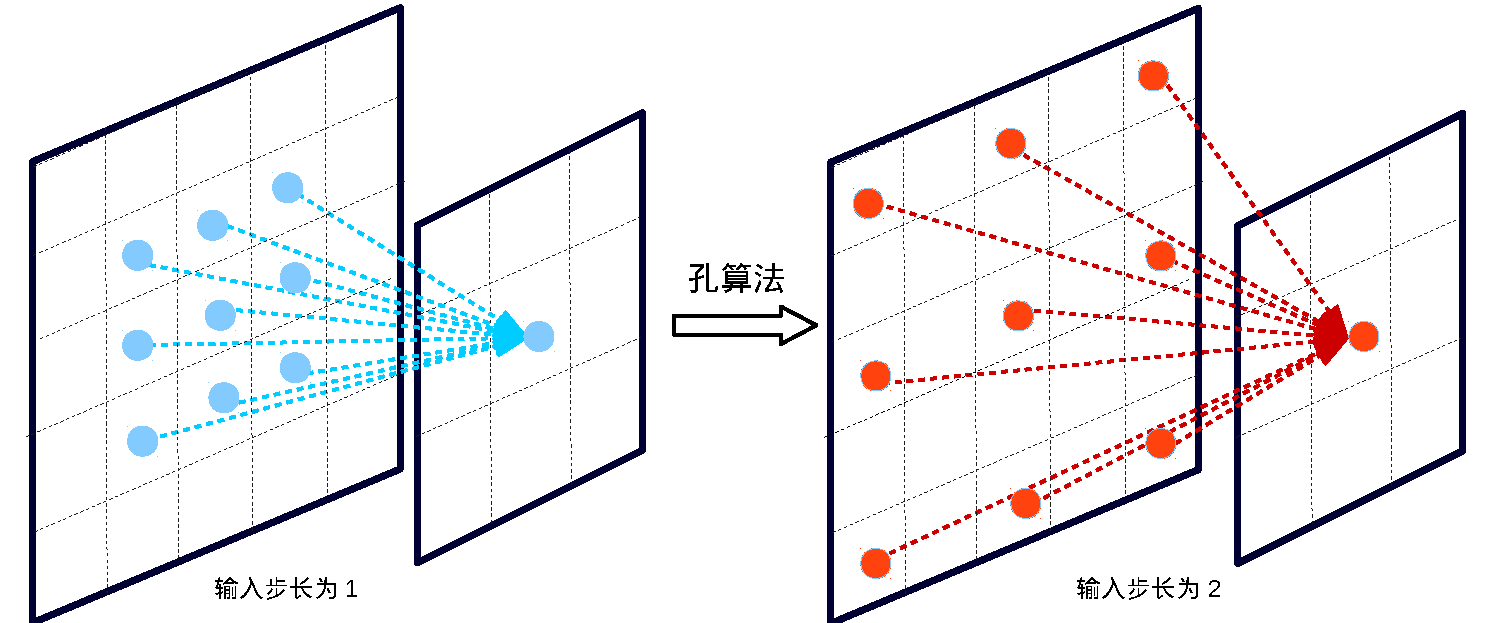
\includegraphics[width=0.5\textwidth]{image/chap04/illustration/hole.pdf}
    \caption{单张图像}
    \label{fig:hole}
\end{figure}


\subsection{多张图像的并排插入}


\begin{figure}[h!]%文中的Grid-LSTM模型做的语义图像分割的例子
    \centering
    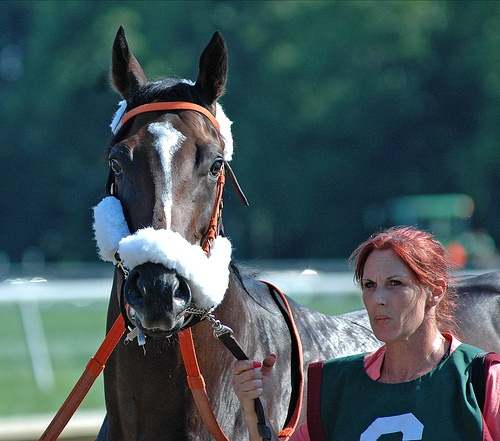
\includegraphics[width=.2\textwidth,height=.15\textwidth]{image/chap04/example/2007_000799.jpg}
    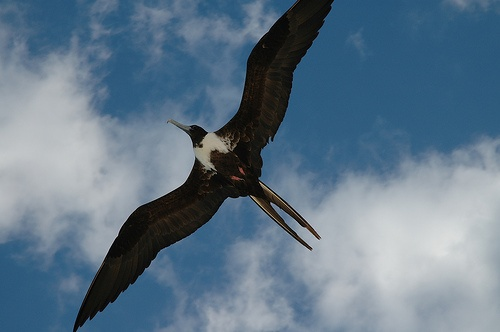
\includegraphics[width=.2\textwidth,height=.15\textwidth]{image/chap04/example/2007_002094.jpg}
    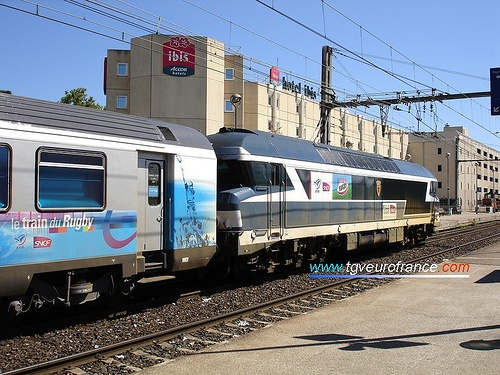
\includegraphics[width=.2\textwidth,height=.15\textwidth]{image/chap04/example/2007_004483.jpg}
    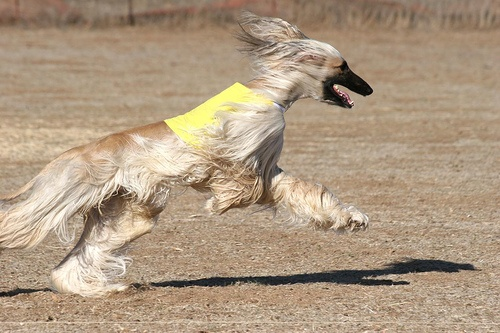
\includegraphics[width=.2\textwidth,height=.15\textwidth]{image/chap04/example/2007_003194.jpg}
    \\
    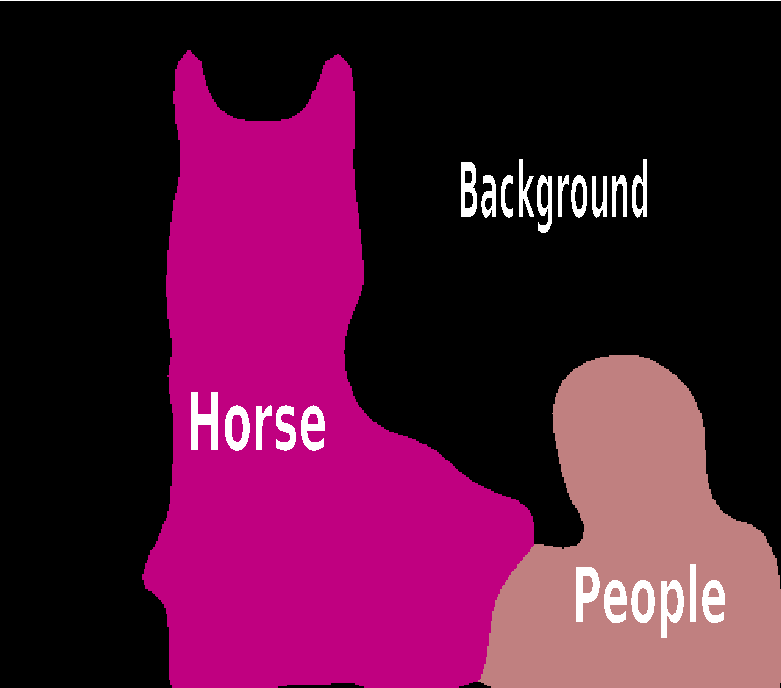
\includegraphics[width=.2\textwidth,height=.15\textwidth]{image/chap04/example/2007_000799.pdf}
    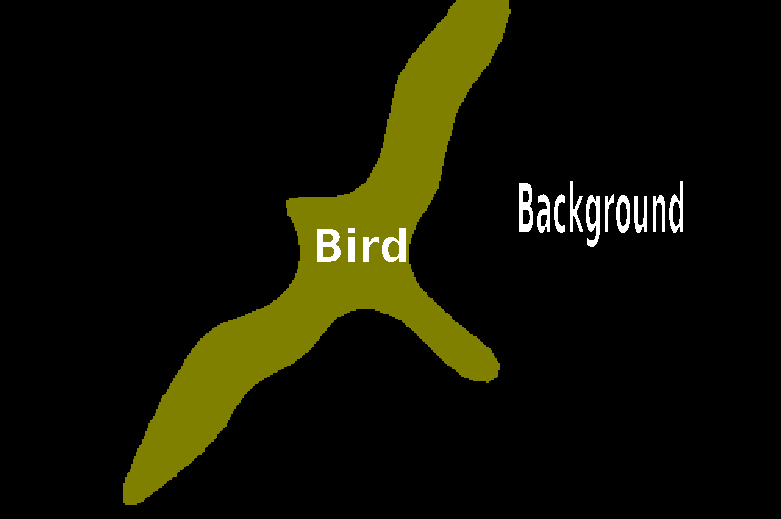
\includegraphics[width=.2\textwidth,height=.15\textwidth]{image/chap04/example/2007_002094.pdf}
    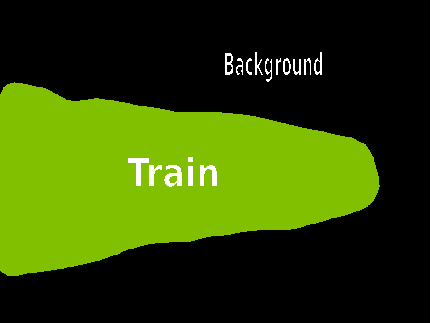
\includegraphics[width=.2\textwidth,height=.15\textwidth]{image/chap04/example/2007_004483.pdf}
    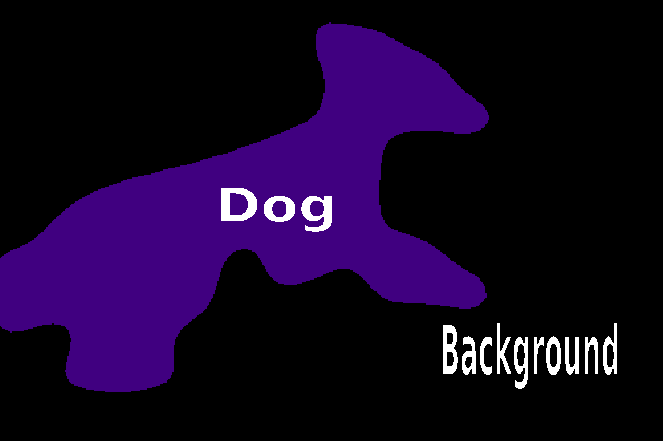
\includegraphics[width=.2\textwidth,height=.15\textwidth]{image/chap04/example/2007_003194.pdf}
    \caption{并排的多张图像}
    \label{fig:multi-image-example1}
\end{figure}


\begin{figure}[h]
    \centering
    \makebox[0.11\textwidth]{\scriptsize 图像}
    \enspace
    \makebox[0.11\textwidth]{\scriptsize 真值}
    \enspace
    \makebox[0.11\textwidth]{\scriptsize CNN+5LSTM\textbf{1}}
    \enspace\thinspace
    \makebox[0.11\textwidth]{\scriptsize CNN+5LSTM\textbf{2}}
    \enspace\thinspace
    \makebox[0.11\textwidth]{\scriptsize CNN+5LSTM\textbf{3}}
    \enspace\thinspace
    \makebox[0.11\textwidth]{\scriptsize CNN+5LSTM\textbf{4}}
    \enspace\thinspace
    \makebox[0.11\textwidth]{\scriptsize CNN+5LSTM\textbf{5}}\\
    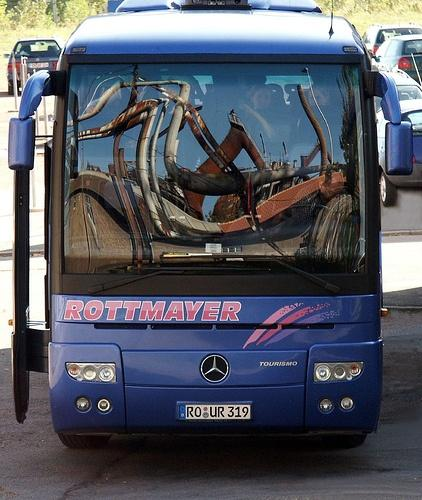
\includegraphics[width=0.11\textwidth]{image/chap04/improvement/2007_000663.jpg}
    \enspace\thinspace %\hfill
    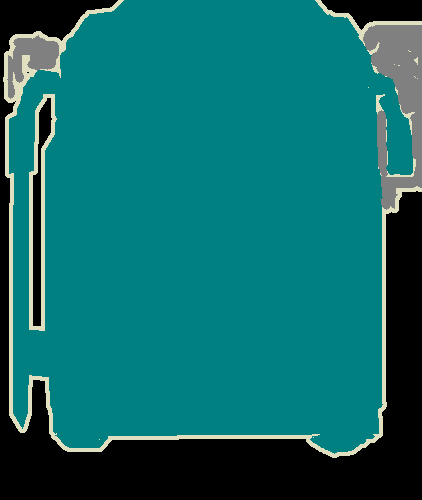
\includegraphics[width=0.11\textwidth]{image/chap04/improvement/2007_000663.png}
    \enspace\thinspace
    
\includegraphics[width=0.11\textwidth]{image/chap04/improvement/2007_000663_1.png}
    \enspace\thinspace
    
\includegraphics[width=0.11\textwidth]{image/chap04/improvement/2007_000663_2.png}
    \enspace\thinspace
    
\includegraphics[width=0.11\textwidth]{image/chap04/improvement/2007_000663_3.png}
    \enspace\thinspace
    
\includegraphics[width=0.11\textwidth]{image/chap04/improvement/2007_000663_4.png}
    \enspace\thinspace
    
\includegraphics[width=0.11\textwidth]{image/chap04/improvement/2007_000663_5.png}
    \enspace\thinspace
    \caption{并排的多张图像加各自的注解}
    \label{fig:improvement}
\end{figure}


\subsection{两列图像的插入}

\begin{figure}[h!] % image examples & compare
    \begin{subfigure}{0.55\textwidth}
        \makebox[0.18\textwidth]{\scriptsize Grid-5LSTM}
        \makebox[0.18\textwidth]{\scriptsize FCN-8s\cite{long2015fully}}
        \makebox[0.18\textwidth]{\scriptsize SDS\cite{hariharan2014simultaneous}}
        \makebox[0.18\textwidth]{\scriptsize 真值}
        \makebox[0.18\textwidth]{\scriptsize 图像} \\
        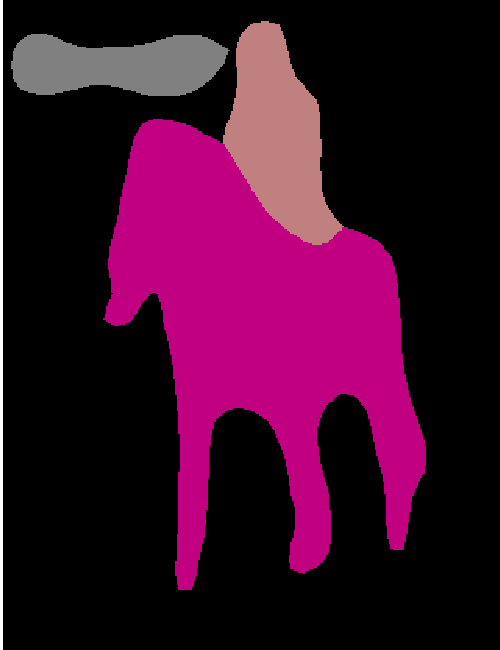
\includegraphics[width=0.18\textwidth]{image/chap04/result/compare/my_horse.pdf}
        
\includegraphics[width=0.18\textwidth]{image/chap04/result/compare/fcn_horse.png}
        
\includegraphics[width=0.18\textwidth]{image/chap04/result/compare/sds_horse.png}
        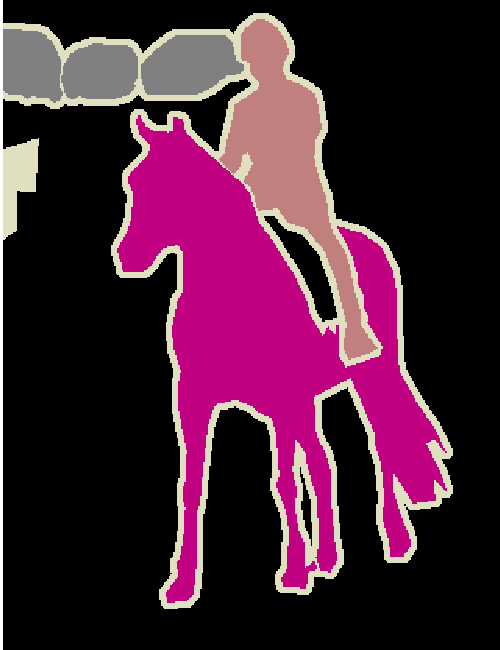
\includegraphics[width=0.18\textwidth]{image/chap04/result/compare/gt_horse.pdf}
        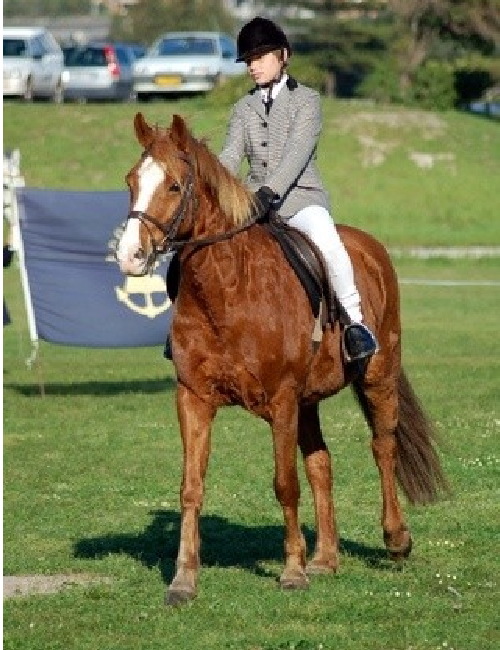
\includegraphics[width=0.18\textwidth]{image/chap04/result/compare/im_horse.pdf}
        \\
        
\includegraphics[width=0.18\textwidth]{image/chap04/result/compare/my_motor.png}
        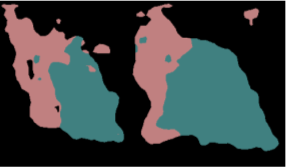
\includegraphics[width=0.18\textwidth]{image/chap04/result/compare/fcn_motor.png}
        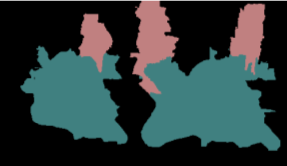
\includegraphics[width=0.18\textwidth]{image/chap04/result/compare/sds_motor.png}
        
\includegraphics[width=0.18\textwidth]{image/chap04/result/compare/2007_005173.png}
        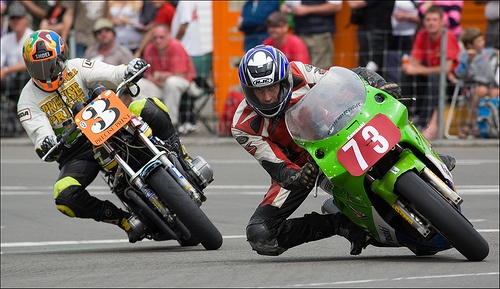
\includegraphics[width=0.18\textwidth]{image/chap04/result/compare/2007_005173.jpg}
        \\
        
\includegraphics[width=0.18\textwidth]{image/chap04/result/compare/my_sheep.pdf}
        
\includegraphics[width=0.18\textwidth]{image/chap04/result/compare/fcn_sheep.png}
        
\includegraphics[width=0.18\textwidth]{image/chap04/result/compare/sds_sheep.png}
        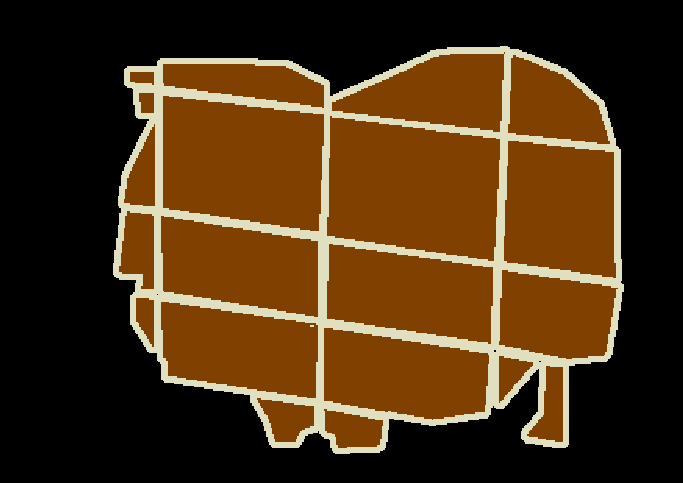
\includegraphics[width=0.18\textwidth]{image/chap04/result/compare/gt_sheep.pdf}
        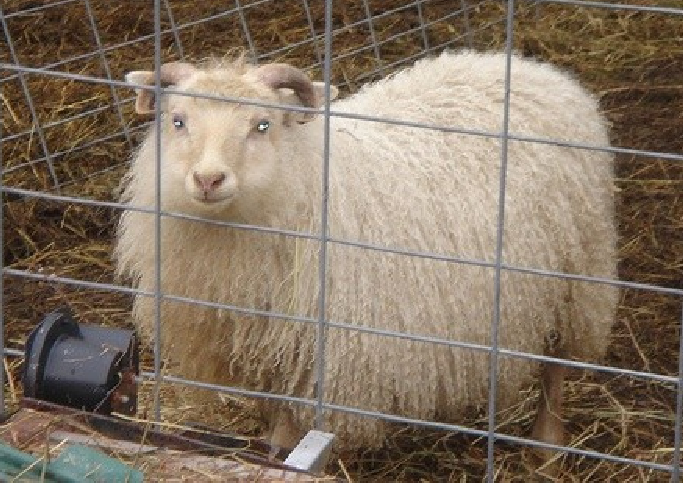
\includegraphics[width=0.18\textwidth]{image/chap04/result/compare/im_sheep.pdf}
        \\
        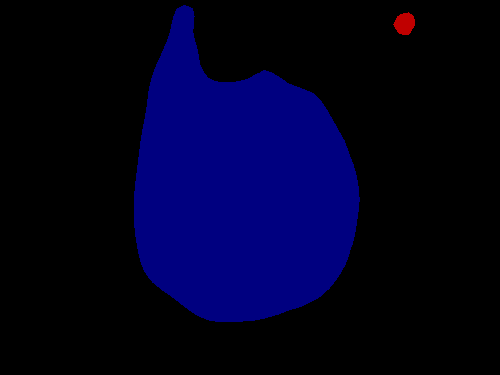
\includegraphics[width=0.18\textwidth]{image/chap04/result/compare/my_boat.png}
        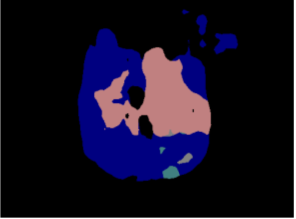
\includegraphics[width=0.18\textwidth]{image/chap04/result/compare/fcn_boat.png}
        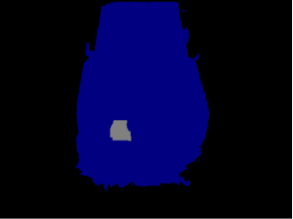
\includegraphics[width=0.18\textwidth]{image/chap04/result/compare/sds_boat.png}
        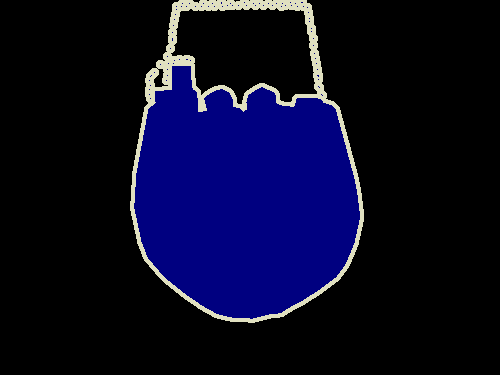
\includegraphics[width=0.18\textwidth]{image/chap04/result/compare/2007_004241.png}
        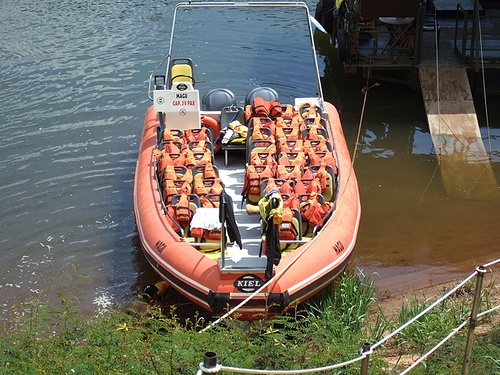
\includegraphics[width=0.18\textwidth]{image/chap04/result/compare/2007_004241.jpg}
        \caption{左边的图像}
        \label{fig:compare1}
    \end{subfigure}
    \begin{subfigure}{0.4\textwidth}
        \centering
        %		\makebox[0.3\textwidth]{} \\
        %		\makebox[0.3\textwidth]{} \\
        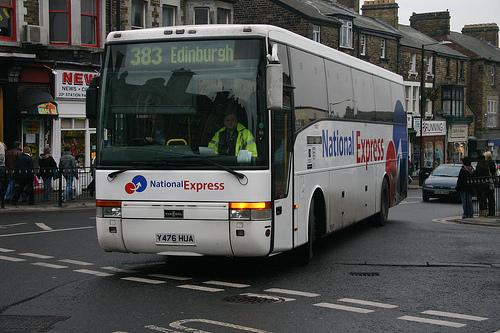
\includegraphics[width=0.25\textwidth]{image/chap04/result/compare/2010_005284.jpg}
        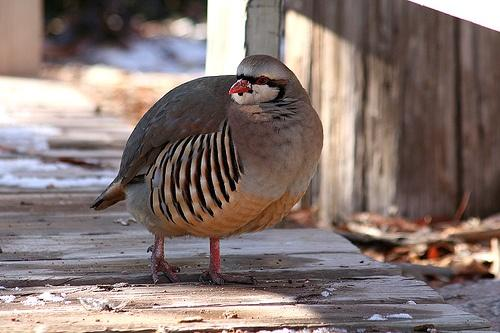
\includegraphics[width=0.25\textwidth]{image/chap04/result/compare/2007_003349.jpg}
        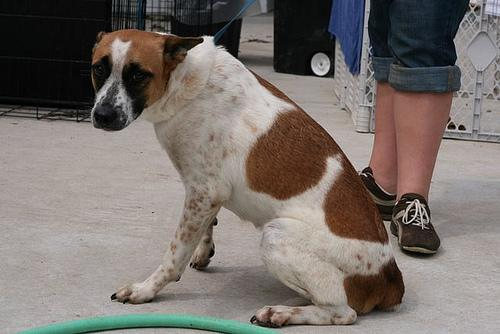
\includegraphics[width=0.25\textwidth]{image/chap04/result/compare/2009_004507.jpg}
        \\
        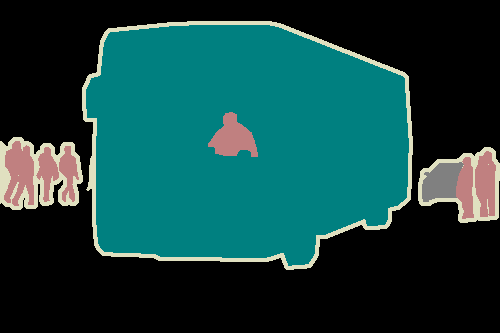
\includegraphics[width=0.25\textwidth]{image/chap04/result/compare/2010_005284.png}
        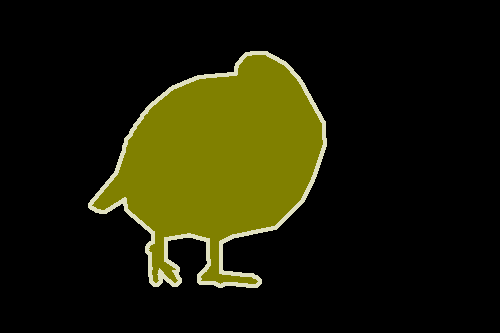
\includegraphics[width=0.25\textwidth]{image/chap04/result/compare/2007_003349.png}
        \includegraphics[width=0.25\textwidth]{image/chap04/result/compare/2009_004507.png} \\
        \includegraphics[width=0.25\textwidth]{image/chap04/result/compare/zoom_bus.png}
        \includegraphics[width=0.25\textwidth]{image/chap04/result/compare/zoom_bird.png}
        \includegraphics[width=0.25\textwidth]{image/chap04/result/compare/zoom_dog.png} \\
        \includegraphics[width=0.25\textwidth]{image/chap04/result/compare/deeplab_bus.png}
        \includegraphics[width=0.25\textwidth]{image/chap04/result/compare/deeplab_bird.png}
        \includegraphics[width=0.25\textwidth]{image/chap04/result/compare/deeplab_dog.png} \\
        \includegraphics[width=0.25\textwidth]{image/chap04/result/compare/my_bus.png}
        \includegraphics[width=0.25\textwidth]{image/chap04/result/compare/my_bird.png}
        \includegraphics[width=0.25\textwidth]{image/chap04/result/compare/my_dog.png}
        \caption{右边的图像}
        \label{fig:compare2}
    \end{subfigure}
    \caption{复杂的两列对象的插入}
    \label{fig:complex}
\end{figure}


\clearpage

\section{表格的插入}

\begin{table}[h] %voc table result
    \centering
    \caption{典型的实验对比表格}
    \begin{tabular}{*{4}{c}}
        \toprule
        Method                                & Pixel Acc.    & Mean Acc.     & Mean Iu.      \\
        \midrule
        Liu等人\cite{liu2011sift}             & 76.7          & -             & -             \\
        Tighe等人\cite{tighe2013finding}      & 78.6          & 39.2          & -             \\
        FCN-16s\cite{long2015fully}           & 85.2          & \textbf{51.7} & 39.5          \\
        Deeplab-LargeFOV\cite{chen14semantic} & 85.6          & 51.2          & 39.7          \\
        \midrule
        Grid-LSTM5                            & \textbf{86.2} & 51.0          & \textbf{41.2} \\
        \bottomrule
    \end{tabular}
    \label{tab:siftflow}
\end{table}

\begin{table}[h] %voc table result
    \centering
    \caption{复杂一些的表格}
    \resizebox{\textwidth}{!}{
        \begin{tabular}{c|*{20}{c}|c}
            \toprule
            Method                    & aero          & bike          & bird          & boat          & bottle        & bus           & car           & cat           & chair         & cow           & table         & dog           & horse         & mbike         & person        & plant         & shep          & sofa          & train         & tv            & mIoU.         \\
            \midrule
            CNN                       & 72.6          & 29.6          & 70.2          & 53.1          & 65.1          & 81.0          & 74.3          & 79.8          & 25.0          & 64.8          & 47.8          & 69.5          & 66.2          & 65.2          & 74.2          & 42.1          & 69.6          & 38.8          & 74.4          & 58.6          & 62.5          \\
            CNN+\textbf{1}LSTM        & 71.5          & 30.6          & 70.5          & 53.8          & 64.9          & 82.4          & 77.1          & 79.5          & 25.1          & 65.8          & 47.8          & 71.5          & 64.6          & 67.0          & 74.0          & 43.9          & 69.6          & 38.6          & 74.9          & 59.4          & 63.0          \\
            CNN+\textbf{2}LSTM        & 76.1          & 32.6          & 72.1          & 57.0          & 65.3          & 83.6          & 75.4          & 81.7          & 24.7          & 69.3          & 47.5          & 72.3          & 68.9          & 69.5          & 74.7          & 41.5          & 69.8          & 38.3          & 77.8          & 62.1          & 64.3          \\
            CNN+\textbf{3}LSTM        & 77.7          & 32.3          & 72.6          & 60.0          & 68.3          & 85.5          & 78.5          & 82.3          & 25.3          & 71.1          & 49.7          & 71.5          & 69.7          & 70.8          & 75.9          & 47.9          & 71.2          & 38.9          & 80.2          & 61.7          & 65.8          \\
            CNN+\textbf{4}LSTM        & 79.1          & \textbf{33.7} & \textbf{73.6} & \textbf{62.0} & \textbf{70.4} & 85.5          & \textbf{80.9} & 83.7          & \textbf{24.1} & 70.7          & 45.7          & 73.7          & 69.6          & 72.1          & 75.6          & 47.2          & \textbf{76.0} & 37.3          & 80.5          & 62.2          & 66.4          \\
            CNN+\textbf{5}LSTM        & \textbf{79.9} & 33.6          & \textbf{73.6} & 61.7          & 68.0          & \textbf{88.5} & \textbf{80.9} & \textbf{84.0} & 23.6          & \textbf{71.3} & \textbf{49.7} & \textbf{73.1} & \textbf{71.3} & \textbf{72.9} & \textbf{76.4} & \textbf{48.9} & 75.1          & \textbf{38.1} & \textbf{84.5} & \textbf{63.8} & \textbf{67.2} \\
            \midrule
            CNN+\textbf{5}LSTM$^\dag$ & 84.8          & 36.4          & 82.0          & 69.4          & 73.0          & 87.2          & 81.8          & 86.1          & 34.5          & 82.4          & 53.1          & 81.5          & 77.4          & 79.0          & 81.3          & 54.8          & 81.1          & 47.0          & 84.3          & 67.3          & 72.3          \\
            \bottomrule
        \end{tabular}}
    \label{tab:vocval}
\end{table}


\section{公式}
\label{sec:formula}
没有编号的公式
\begin{align*}
    \begin{split}
        \label{eq:feedforward}
        \mybold{z}^{(l)} & = \mybold{W}^{(l)}\mybold{a}^{(l-1)} + \mybold{b}^{(l)} \\
        \mybold{a}^{(l)} & = f(\mybold{z}^{(l)})
    \end{split}
\end{align*}
公式中含有中文
\begin{align}
    \begin{split}
        \mbox{像素准确率} &= \sum_{i=1}^{n_{cl}}n_{ii} / \sum_{i=1}^{n_{cl}}t_i \\
        \mbox{平均像素准确率} &= \frac{1}{n_{cl}} \sum_{i=1}^{n_{cl}}(n_{ii}/ t_i) \\
        \mbox{Mean IU} &= \frac{1}{n_{cl}} \sum_{i=1}^{n_{cl}}\frac{n_{ii}}{t_i + \sum_j^{n_{cl}} n_{ji} - n_{ii}}
    \end{split}
\end{align}
公式中含有矩阵
\begin{equation}
    \textbf{H} = \begin{bmatrix}
        I*\mybold{x}_i \\ \textbf{h}
    \end{bmatrix}
\end{equation}
每行后面都有编号的公式
\begin{align}
    \frac{\partial}{\partial W_{ij}^{(l)}} J(\mybold{W},\mybold{b};\mybold{x},y) & = \frac{\partial J(\mybold{W},\mybold{b};\mybold{x},y)}{\partial z_i^{(l+1)}}\cdot \frac{\partial z_i^{(l+1)}}{\partial W_{ij}^{(l)}} = \delta_i^{(l+1)}a_j^{(l)} \\
    \frac{\partial}{\partial b_i^{(l)}} J(\mybold{W},\mybold{b};\mybold{x},y)    & = \frac{\partial J(\mybold{W},\mybold{b};\mybold{x},y)}{\partial z_i^{(l+1)}}\cdot \frac{\partial z_i^{(l+1)}}{\partial b_i^{(l)}} = \delta_i^{(l+1)}
\end{align}

\section{算法流程图}
\label{sec:algorithm}
\begin{algorithm}[h]
    \KwIn{$m$个训练样本}
    \lFor{$l=1$ \emph{\KwTo} $n_l$}{
        初始化:$\Delta \mybold{W}^{(l)}=0$,$\Delta \mybold{b}^{(l)}=0$}
    \ForEach{训练样本}{
        \lFor{$l=1$ \emph{\KwTo} $n_l-1$}{
            前向传播:$\mybold{z}^{(l+1)}=\mybold{W}^la^l+\mybold{b}^l$,$\mybold{a}^{(l+1)}=f(\mybold{z}^{(l+1)})$}
        输出误差计算:$\delta^{(n_l)} = \frac{\partial}{\partial \mybold{z}^{(n_l)}} J(\mybold{W},\mybold{b};\mybold{x},y)$\;
        \lFor{$l=n_l-1$ \emph{\KwTo} $1$}{
            后向传播:$\delta^{(l)} = \bigl((\mybold{W}^{(l)})^T \delta^{(l+1)}\bigr)f'(\mybold{z}^{(l)})$}
        \ForAll{层l}{
            计算梯度:$\nabla_{\mybold{W}^{(l)}}J(\mybold{W},\mybold{b};\mybold{x},y)=\delta^{(l+1)}(\mybold{a}^{(l)})^T$ \\
            \hspace{60pt}$\nabla_{\mybold{b}^{(l)}}J(\mybold{W},\mybold{b};\mybold{x},y)=\delta^{(l+1)}$\;
            累加梯度:$\Delta \mybold{W}^{(l)} \leftarrow \Delta \mybold{W}^{(l)} + \nabla_{\mybold{W}^{(l)}}J(\mybold{W},\mybold{b};\mybold{x},y)$; \\
            \hspace{60pt}$\Delta \mybold{b}^{(l)} \leftarrow \Delta \mybold{b}^{(l)} + \nabla_{\mybold{b}^{(l)}}J(\mybold{W},\mybold{b};\mybold{x},y)$\;
        }
    }
    \ForAll{层$l$}{
        更新权重:$\mybold{W}^{(l)} \leftarrow \mybold{W}^{(l)} - \alpha \biggl[\frac 1m \Delta \mybold{W}^{(l)}\biggr]$ \\
        \hspace{60pt} $\mybold{b}^{(l)} \leftarrow \mybold{b}^{(l)} - \alpha \biggl[\frac 1m \Delta \mybold{b}^{(l)}\biggr]$
    }
    \caption{梯度下降算法}
    \label{algo:sgd}
\end{algorithm}

\section{例子、定理与证明}

\begin{eg}
    这是一个例子, 用以验证特殊环境的字体成功更改为楷体.
\end{eg}

\begin{theorem}[定理例子]
    \label{the:example-theorem}
    这是一个定理。
\end{theorem}

\begin{corollary}[推论例子]
    \label{the:example-corollary}
    这是一个推论。
\end{corollary}

\begin{lemma}[引理例子]
    \label{the:example-lemma}
    这是一个引理。
\end{lemma}

这里我们先给出\autoref{the:example-theorem-sysu-thesis}

\begin{theorem}[中山大学毕业论文模板定理]
    \label{the:example-theorem-sysu-thesis}
    中山大学 \LaTeX 毕业论文模板可以用于写各种证明。
\end{theorem}

下面我们对\autoref{the:example-theorem-sysu-thesis}进行证明:


\begin{proof}

    下面我们开始证明:

    由本定理的证明可见,我可以引用\autoref{the:example-theorem}和引理\ref{the:example-corollary}以及推论\ref{the:example-lemma}来证明我这个 \LaTeX 可以用来写各种证明。 \\

    \autoref{the:example-theorem-sysu-thesis}得证。
\end{proof}

\section{代码}

本模版支持在论文中插入代码片段,或直接从源码文件进行插入。
例如,在论文中插入代码片段的效果为:
\begin{python}
    def func():
    print("hello world")
    with open('./output.txt', 'w') as f:
    L = f.readlines()

    if __name__ == "__main__":
    # this is a comment line
    func()
\end{python}
也可在行内插入代码片段,例如:Python中重载加法运算符的函数为\pyinline{__add__},类的标识符为\pyinline{class}。
此外,还可直接插入代码文件,例如插入\texttt{./code/demo.cpp}的效果为:
\lstinputlisting[style=sysucpp]{code/demo.cpp}


\section{其他的一些用法}
\label{sec:font}
\subsection{子章节编号}
\label{sec:font:subsection}
\subsubsection{更小的章节}
\label{sec:font:subsection:subsub}
更小的章节编号也是支持的。

可以如此引用章节:

\begin{itemize}
    \item \autoref{cha:usage-example}
    \item  \autoref{sec:font}
    \item  \autoref{sec:font:subsection}
    \item  \autoref{sec:font:subsection:subsub}
\end{itemize}


\subsection{列表的使用}
\label{sec:font:list}

这是一个无序列表
\begin{itemize}
    \item 引用文献
    \item 引用文献作者
    \item 引用文献年份
    \item 字体{\color{red}{变红}},\textbf{粗体},\textit{斜体},\underline{下划线}。
\end{itemize}

这是一个有序列表
\begin{enumerate}
    \item 索引前面的\autoref{sec:formula}、图像\ref{fig:complex}、表格\ref{tab:siftflow}
    \item 加脚注\footnote{测{\zihao{-5}试一下}脚注和URL \url{http://cs231n.github.io/transfer-learning/}}
\end{enumerate}



\newclearpage
% %% chapter 5 dataset, network structure, experiment and result
\chapter{实验与结果}
\label{cha:experiment}

\section{关于生僻字}

测试生僻字

昇䊒熗庈焾燋庼廎㶭粌纇颣炥䊧彂㢕糑鄜麛麚䴫麌䴠麎塵䴣麆麠䴤麖䴨䴩䴪麘麞麡麍麏麐麔	

% \newclearpage

% 结语

% 附录部分
\backmatter
% 参考文献. 因不需要纳入章节目录, 故放入附录部分
% 实际上参考文献是属于论文主体部分
\makereferences

% 附录
{
    \appendix
    \chapter{证明细节}
\section{生成对抗网络损失函数推导}
记$l$是样本$x$的真实标签,而$y$则是神经网络判别器$D$给出的认为真样本的可能性,$y=D(\mathbf{x})$
从判别器$D$的角度对某个样本i考虑
$$L_i=y_i^{l_i}(1-y_i)^{(1-l_i)}$$
如果$l_i=1$,上式为$L_i=y_i$,显然$y_i$预测为真的概率越大,预测越正确,$L_i$越大
同理若$l_i=0$,上式为$L_i=1-y_i$,$y_i$预测为真的概率越大,预测越错,$L_i$越小
因此考虑将GAN判别器$D$损失问题转变为极大似然估计问题,如何在一批样本$\{x_1,x_2,...,x_m\}$训练后,最大化预测正确率$L$
%无标号的公式
\begin{align*}
        \underset{D}{max}L=\prod_{i=1}^mL_i=\prod_{i=1}^my_i^{l_i}(1-y_i)^{1-l_i}
\end{align*}
做数学变化,引入单调函数$\log$,并做常见的平均处理,问题转换为等价的优化问题
\begin{align*}
    \begin{split}
        \underset{D}{max}\frac{1}{m}\sum_{i=1}^m\Big[\log y_i^{l_i}+\log(1-y_i)^{1-l_i}\Big] \\
        \underset{D}{max}\frac{1}{m}\sum_{i=1}^m\Big[l_i\log D(x_i)+(1-l_i)D(x_i)\Big]
    \end{split}
\end{align*}
由于标签只有在$x\sim p_{data}(x)$时为1,在$z\sim p_{seed}(x)$时为0,因此上式是期望的样本实现。我们将标签为假的样本写成有生成器输出结果$G(z)$
\begin{align*}
    \begin{split}
        \underset{D}{max}\Big[\mathbb{E}_{x\sim p_{data}(x)}\log D(x)+\mathbb{E}_{z\sim p_{seed}(x)}\big(1-D(G(z))\big)\Big]
    \end{split}
\end{align*}
上式只是对判别器$D$建立了优化目标,显然判别器越强,生成器生成的样本就永远会高概率判断为假。因此生成器的目标是最小化判别器的优化目标
\begin{align*}
    \begin{split}
        \underset{G}{min}\underset{D}{max}\Big[\mathbb{E}_{x\sim p_{data}(x)}\log D(x)+\mathbb{E}_{z\sim p_{seed}(x)}\big(1-D(G(z))\big)\Big]
    \end{split}
\end{align*}
假设生成器$G$有网络参数$\mathbf{\phi}$,判别器$D$有网络参数$\mathbf{\theta}$,我们可以从网络参数的角度给出最终的损失函数

\begin{equation}
    \underset{G}{min}\underset{D}{max}\Big[\mathbb{E}_{x\sim p_{data}(x,\phi)}\log D(x)+\mathbb{E}_{z\sim p_{seed}(x)}\big(1-D(G(z,\theta),\phi)\big)\Big]
\end{equation}

\section{扩散模型正向过程推导部分}
参考\cite{luo2022understanding}\cite{weng2021diffusion}
在扩散模型的前向过程中,来自训练集的图像$\mathbf{x}_0$会被添加$T$次噪声,
使得$\mathbf{x}_T$为符合标准正态分布。大多数前向过程采样的正态分布会设置为下式
\begin{align*}
    \mathbf{x}_t\sim\mathcal{N}(\sqrt{1-\beta_t}\mathbf{x}_{t-1},\beta_t\mathbf{I})
\end{align*}
尝试从$\mathbf{x}_t$持续倒推,$\mathbf{x}_t$可以通过一个标准正态分布的样本$\epsilon_{t-1}\sim\mathcal{N}(0,\mathbf{I})$算出来:
\begin{align*}
    \begin{split}
        \mathbf{x}_t=\sqrt{1-\beta_t}\mathbf{x}_{t-1}+\sqrt{\beta_t}\epsilon_{t-1}\\
        \mathbf{x}_t=\sqrt{1-\beta_t}\Big(\sqrt{1-\beta_{t-1}}\mathbf{x}_{t-2}+\sqrt{\beta_{t-1}}\epsilon_{t-2}\Big)+\sqrt{\beta_t}\epsilon_{t-1}\\
        \mathbf{x}_t=\sqrt{(1-\beta_t)(1-\beta_{t-1})}\mathbf{x}_{t-2}+\sqrt{(1-\beta_t)\beta_{t-1}}\epsilon_{t-2}+\sqrt{\beta_T}\epsilon_{t-1}
    \end{split}
\end{align*}
服从相同均值的正态分布的两个随机向量之和所服从的分布,均值不变但方差是原随机变量方差之和。我们可以改写上式为
\begin{align*}
    \begin{split}
        =\sqrt{(1-\beta_t)(1-\beta_{t-1})}\mathbf{x}_{t-2}+\sqrt{(1-\beta_t)\beta_{t-1}+\beta_t}\epsilon\\
        =\sqrt{(1-\beta_t)(1-\beta_{t-1})}\mathbf{x}_{t-2}+\sqrt{1-(1-\beta_t)(1-\beta_{t-1})}\epsilon
    \end{split}
\end{align*}
将这样的过程一直推到$\mathbf{x}_0$,令$\alpha_t=1-\beta_t,\bar{\alpha}_t=\Pi_{i=1}^t\alpha_i$,则有
\begin{equation}
    \mathbf{x}_t=\sqrt{\bar{\alpha}_t}\mathbf{x}_0+\sqrt{1-\bar{\alpha}_t}\epsilon
\end{equation}
在DDPM的论文中,当$\beta_t$从$\beta_1=10^{-4}$到$\beta_T=0.02$线性增长,$\alpha_t$越来越小,$\bar{\alpha}_t$趋向于0的速度越来越快。
到最后的$T$时刻$\bar{\alpha}_T$几乎为0,这也使得$\mathbf{x}_T=\sqrt{\bar{\alpha}_T}\mathbf{x}_0+\sqrt{1-\bar{\alpha}_T}\epsilon$满足标准正态分布,
以符合扩撒模型加噪声的需求:从慢到快的改变原图像,让图像最终均值为$0$,方差为$\mathbf{I}$

\section{扩散模型加噪声逆操作均值和方差的推导}
在加噪声逆操作的数学推导部分,综合贝叶斯公式得到了
\begin{align*}
    q(x_{t-1}|x_t,x_0)=\mathcal{N}(x_{t-1};\tilde{\mu}_t,\tilde{\beta}_t\mathbf{I})
\end{align*}

    \newclearpage
}

%%
% 致谢
% 谢辞应以简短的文字对课题研究与论文撰写过程中曾直接给予帮助的人员(例如指导教师、答疑教师及其他人员)表示对自己的谢意,这不仅是一种礼貌,也是对他人劳动的尊重,是治学者应当遵循的学术规范。内容限一页。
% modifier: 黄俊杰
% update date: 2017-04-15
%%

\chapter{致谢}

四年时间转眼即逝,青涩而美好的本科生活快告一段落了。回首这段时间,我不仅学习到了很多知识和技能,而且提高了分析和解决问题的能力与养成了一定的科学素养。虽然走过了一些弯路,但更加坚定我后来选择学术研究的道路,实在是获益良多。这一切与老师的教诲和同学们的帮助是分不开的,在此对他们表达诚挚的谢意。

首先要感谢的是我的指导老师王大明教授。我作为一名本科生,缺少学术研究经验,不能很好地弄清所研究问题的重点、难点和热点,也很难分析自己的工作所能够达到的层次。王老师对整个研究领域有很好的理解,以其渊博的知识和敏锐的洞察力给了我非常有帮助的方向性指导。他严谨的治学态度与辛勤的工作方式也是我学习的榜样,在此向王老师致以崇高的敬意和衷心的感谢。

最后我要感谢我的家人,正是他们的无私的奉献和支持,我才有了不断拼搏的信心和勇气,才能取得现在的成果。

\vskip 108pt
\begin{flushright}
	何宇\makebox[1cm]{} \\
	\today
\end{flushright}

    % 致谢
\newclearpage

% \makeGrade      % 成绩评定记录表
\end{document}
